\chapter{Results and Conclusions}

%This section should discuss issues you encountered as you tried to implement your experiments. What were the results of running the experiments? What conclusions can you draw from these results? 
%
%During the work, you might have found that elements of your experiments were unnecessary or overly complex; perhaps third party libraries were available that simplified some of the functions that you intended to implement. If things were easier in some areas, then how did you adapt your project to take account of your findings?
%
%It is more likely that things were more complex than you first thought. In particular, were there any problems or difficulties that you found during implementation that you had to address? Did such problems simply delay you or were they more significant? 
%
%If you had multiple experiments to run, it may be sensible to discuss each experiment in separate sections. 

This chapter presents the key results from the three primary experiments conducted under the investigation for this project. 

\clearpage
\section{Investigation Results}

\subsection{Experiment 1: Template Matching (Overlapping Small Patches)}

\subsubsection{Dataset 1: Living Room Carpet (Indoors)}

\begin{figure}[ht!]
\centering
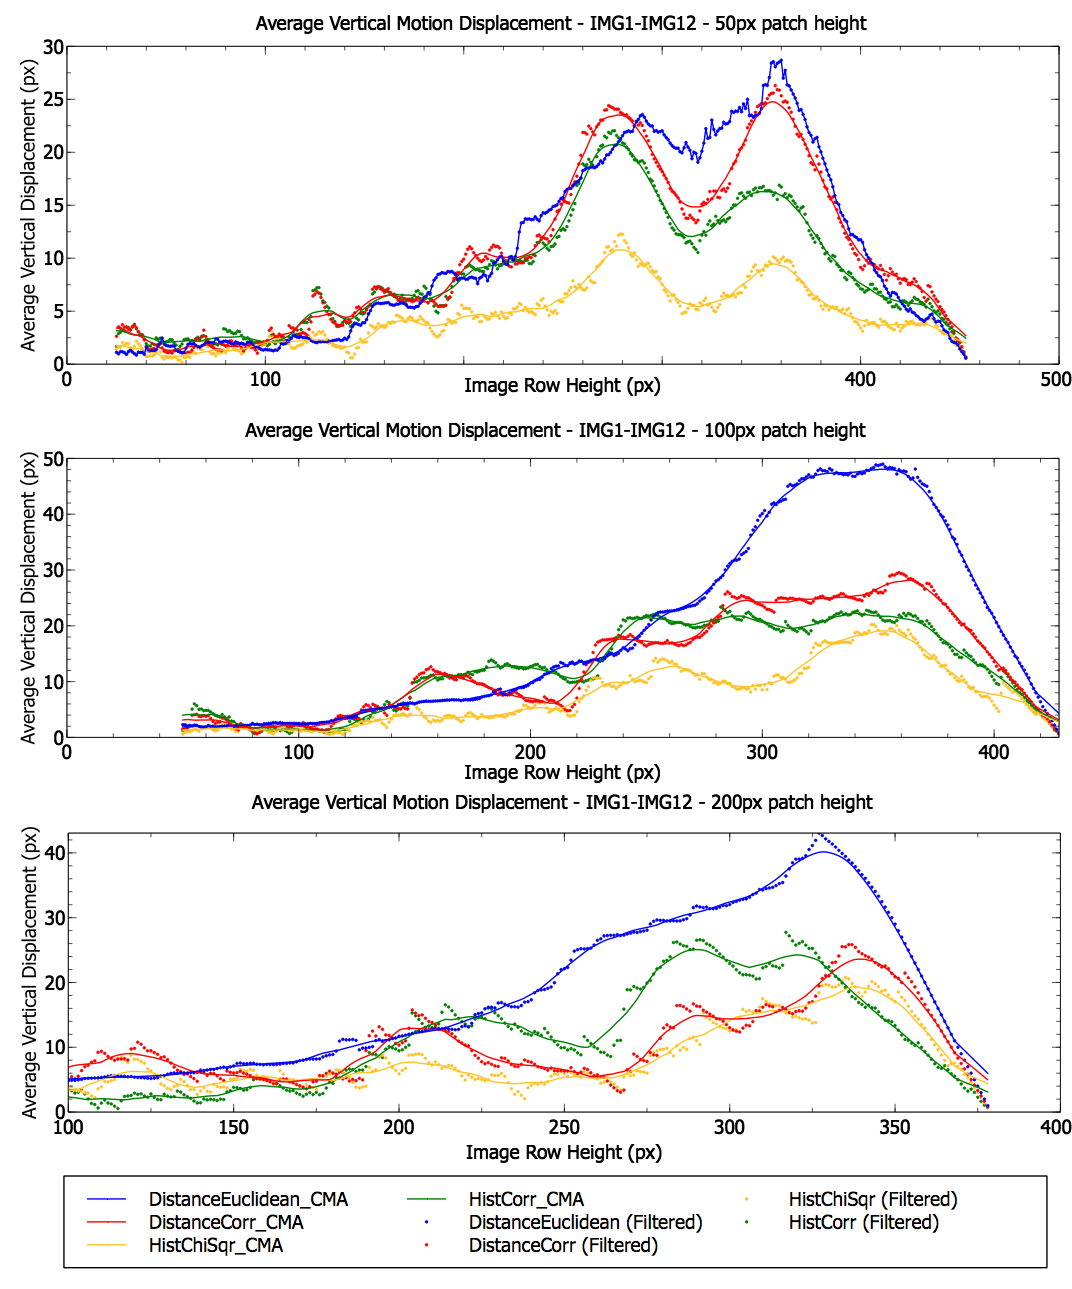
\includegraphics[scale=0.4]{images/results/ex1_results_flat_10cm}
\caption{Average vertical motion displacement models across all images within ``living room carpet" dataset running \textit{non-exhaustive} localised search. Graph 1 (Top) - Overlapping patches of 50px-square; Graph 2 (Middle) Overlapping patches of 100px-square; Graph 3 (Bottom) Overlapping patches of 200px-square. Solid line indicates centred moving average (10-pixel interval) calculated from filtered results for each image similarity metric.}
\label{fig:ex1_1_1}
\end{figure}

The results within Figure \ref{fig:ex1_1_1} indicate an increase between the position of matched features along the vertical axis of the image, and the subsequent vertical displacement that is demonstrated between two consecutive images. While this trend is visible across all three patch sizes, the maximum displacement is recorded using the 100px patch size. Out of the four similarity metrics, Euclidean Distance appears to show the best performance across all of the  patch sizes.

\clearpage
\subsubsection{Dataset 2: Brick-Paved Road (Outside)}

\begin{figure}[ht!]
\centering
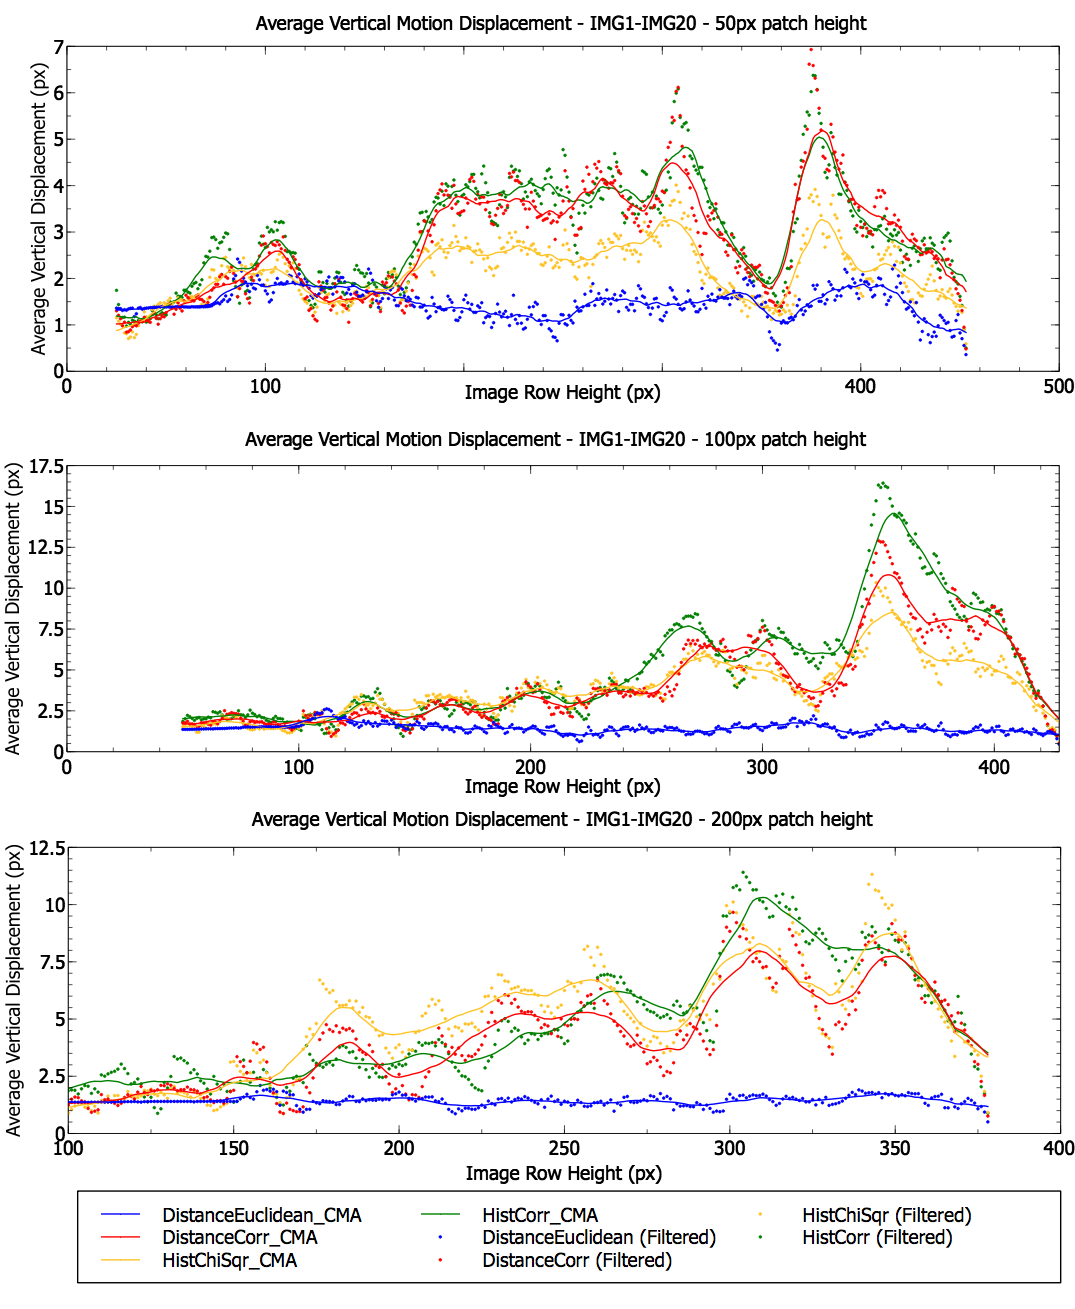
\includegraphics[scale=0.4]{images/results/ex1_results_outside_10cm}
\caption{Average vertical motion displacement models across all images within ``brick-paved road" dataset running \textit{non-exhaustive} localised search. Graph 1 (Top) - Overlapping patches of 50px-square; Graph 2 (Middle) Overlapping patches of 100px-square; Graph 3 (Bottom) Overlapping patches of 200px-square. Solid line indicates centred moving average (10-pixel interval) calculated from filtered results for each appearance-based template matching similarity metric.}
\label{fig:ex1_1_2}
\end{figure}

For dataset two, the results show while there does still appear to be an overall positive correlation shown in Figure \ref{fig:ex1_1_1}, across all three patch sizes it is much weaker and with a significant level of distortion. While the two histogram-based similarity measures and Normalised Cross-Correlation all provided similar results, the Euclidean Distance appears to consistently fail in identifying any significant displacement. Interestingly, Graph 1 shows how all three of the better-performing similarity measures suddenly report a dip in displacement at around row 300, before returning again just before row 400. (\ref{fig:ex1_1_2}).

\clearpage
\subsubsection{Dataset 3: Asian Rug (Indoors)}

\begin{figure}[ht!]
\centering
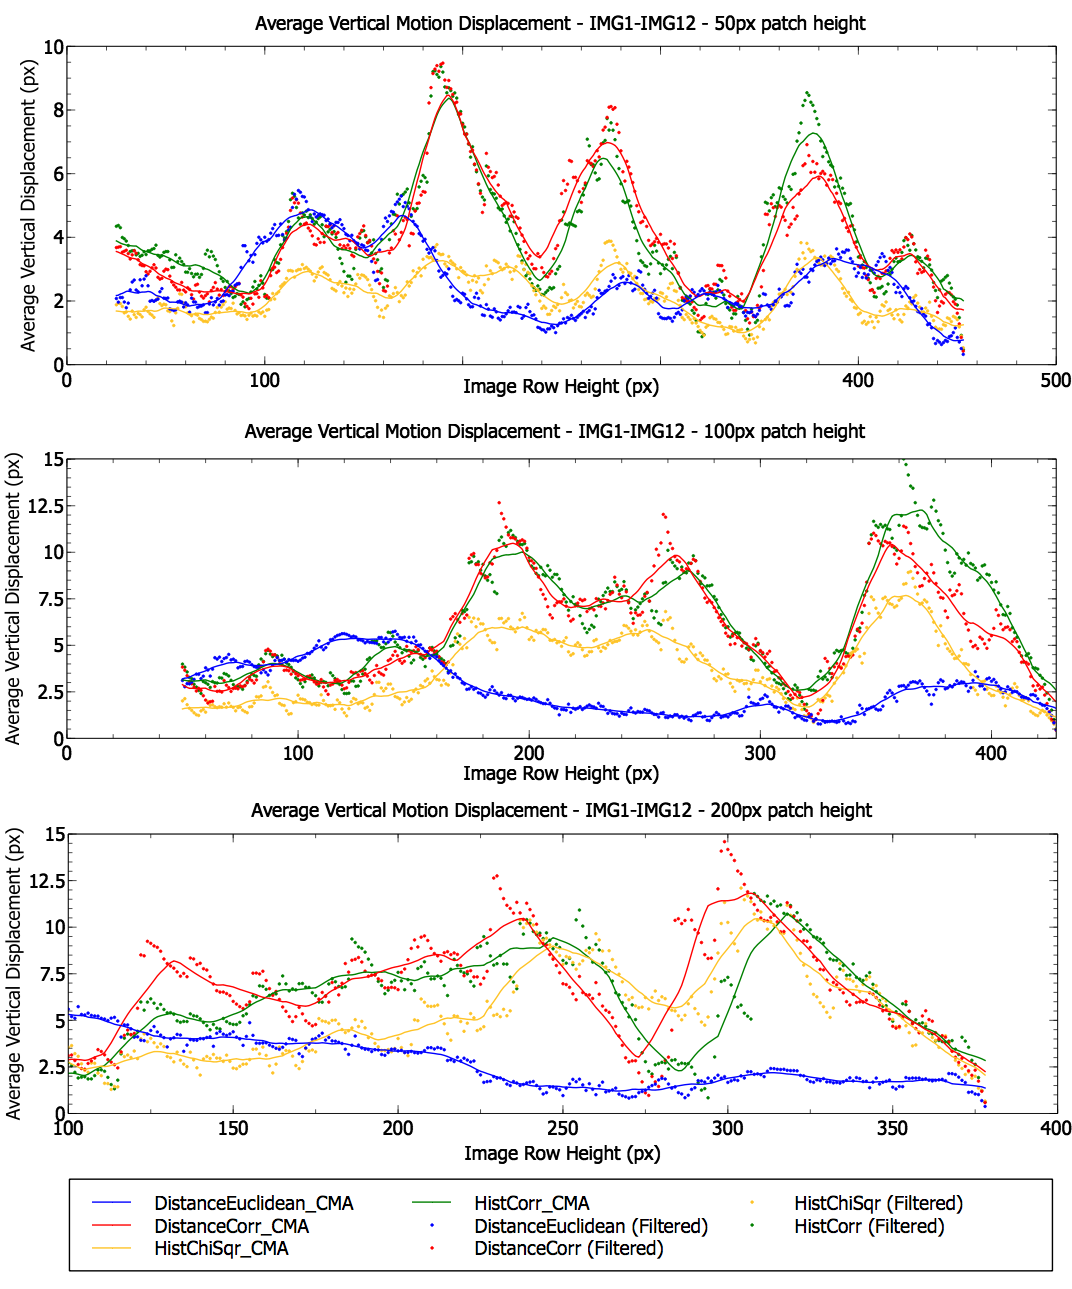
\includegraphics[scale=0.4]{images/results/ex1_results_inside_10cm}
\caption{Average vertical motion displacement models across all images within ``asian rug" dataset running \textit{non-exhaustive} localised search. Graph 1 (Top) - Overlapping patches of 50px-square; Graph 2 (Middle) Overlapping patches of 100px-square; Graph 3 (Bottom) Overlapping patches of 200px-square. Solid line indicates centred moving average (10-pixel interval) calculated from filtered results for each appearance-based template matching similarity metric.}
\label{fig:ex1_1_3}
\end{figure}

Within the results for dataset three (Figure \ref{fig:ex1_1_3}), the vertical displacement shown Graph 1 (50px patch) demonstrates a high level of distortion with no distinct correlation with the vertical height of the row within the image. While the results within Graphs 2 and 3 also demonstrate no particular positive correlation between the row within the image, and the vertical displacement that is demonstrated, they do both appear to identify a sudden decrease in displacement at the same vertical height in the image (approx. 275px for 100px patch and 350px for 200px patch).

\clearpage
\subsubsection{Dataset 4: Slate Footpath (Outdoors)}

\begin{figure}[ht!]
\centering
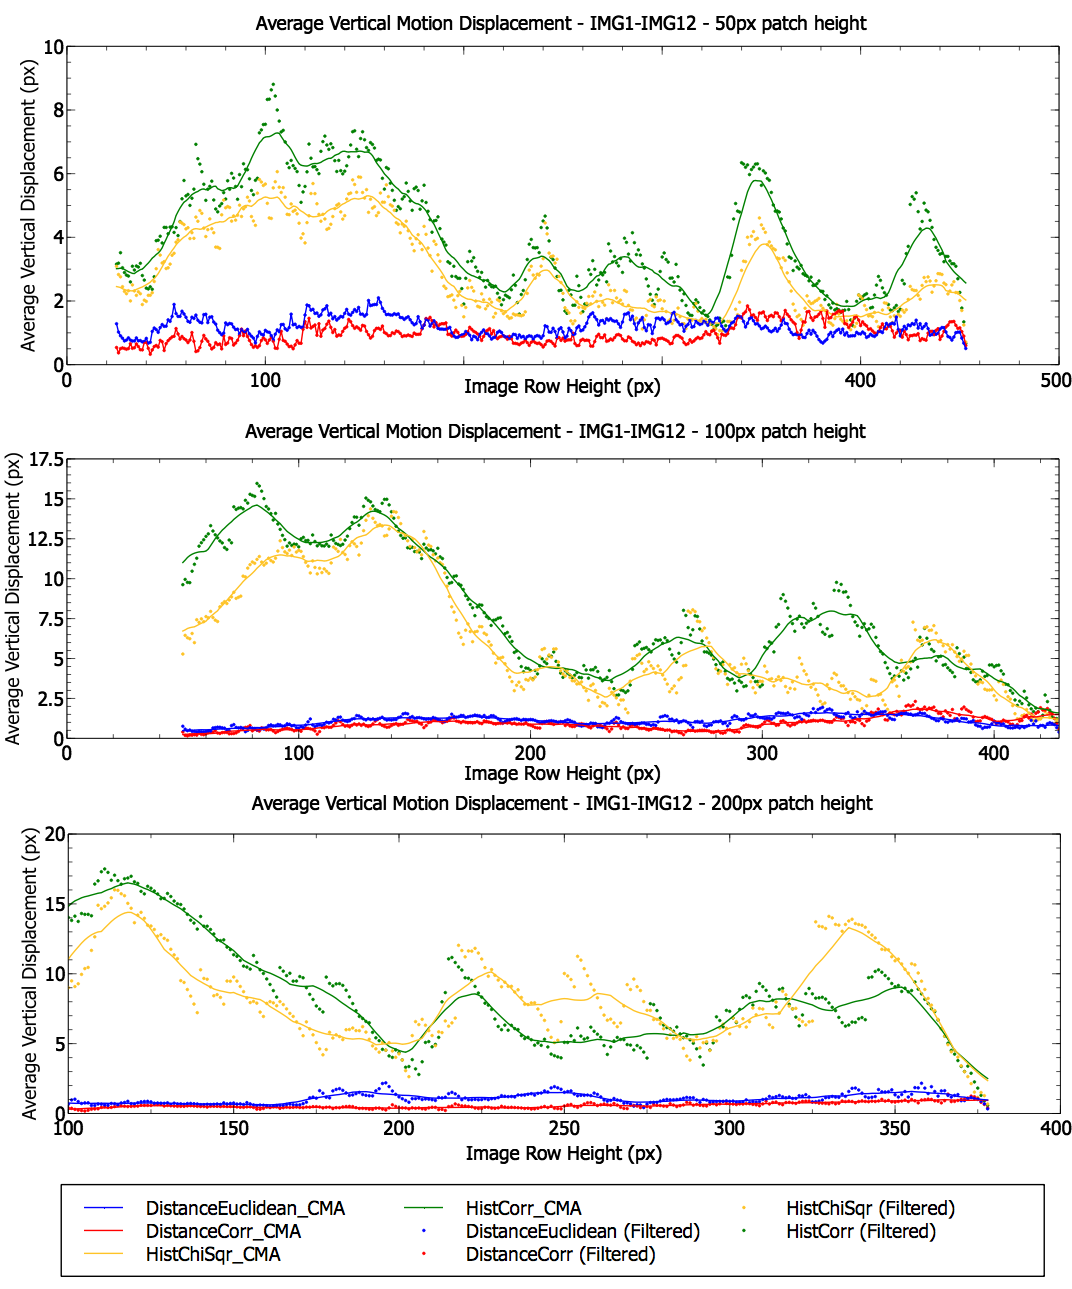
\includegraphics[scale=0.4]{images/results/ex1_results_path_outside_10cm}
\caption{Average vertical motion displacement models across all images within ``slate footpath" dataset running \textit{non-exhaustive} localised search. Graph 1 (Top) - Overlapping patches of 50px-square; Graph 2 (Middle) Overlapping patches of 100px-square; Graph 3 (Bottom) Overlapping patches of 200px-square. Solid line indicates centred moving average (10-pixel interval) calculated from filtered results for each appearance-based template matching similarity metric.}
\label{fig:ex1_1_4}
\end{figure}


The results within Figure \ref{fig:ex1_1_4}, the tests across all three patch sizes appear to indicate similar results, with a clear divide visible between the performance of the histogram-based, and distance-based similarity measures. Of particular interest is the unexpected negative-correlation trend recorded by the histogram-based similarity measures that appears within all three of the graphs, potentially indicate an issue within the dataset.


\clearpage
\subsection{Experiment 2: Template Matching (Full-width Patches - Non-Scaled)}

\subsubsection{Dataset 1: Living Room Carpet (Indoors)}

\begin{figure}[ht!]
\centering
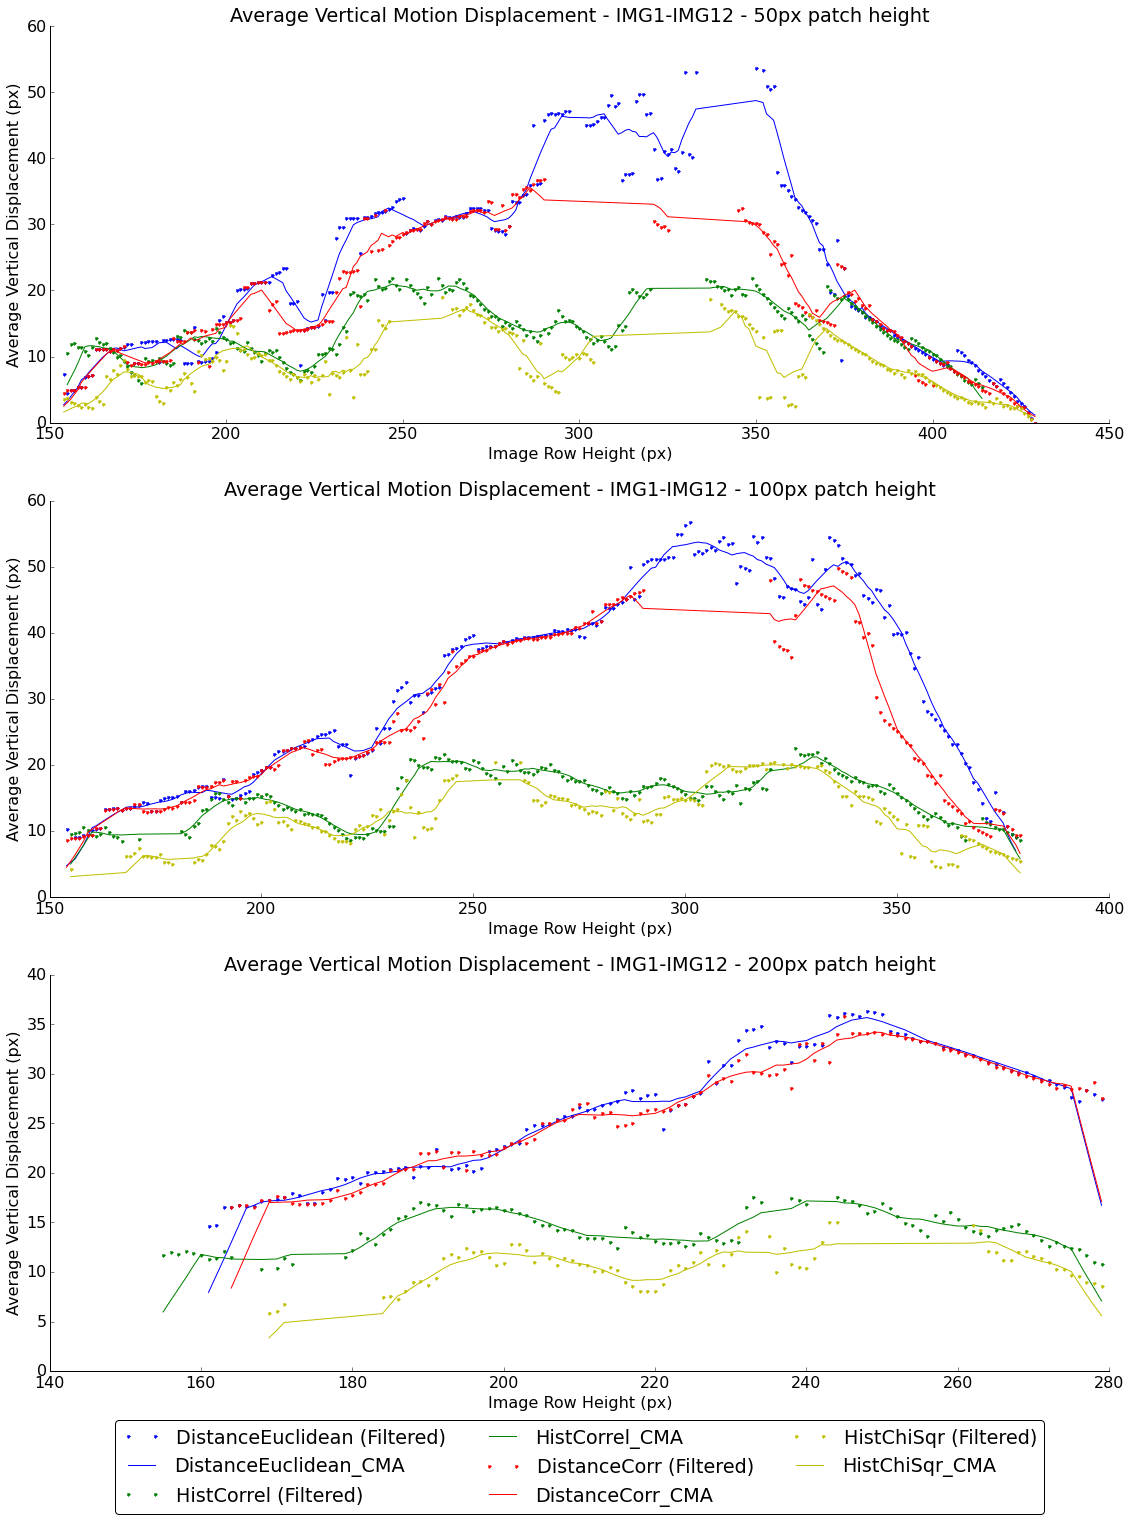
\includegraphics[scale=0.3]{images/results/flat_10cm_non_scaled}
\caption{Average vertical motion displacement models across all images within ``living room carpet" dataset running \textit{non-exhaustive} localised search. Graph 1 (Top) - Full-width patch with fixed height of 50px; Graph 2 (Middle) Full-width patch with fixed height of 100px; Graph 3 (Bottom) Full-width patch with fixed height of 200px. Solid line indicates centred moving average (10-pixel interval) calculated from filtered results for each appearance-based template matching similarity metric.}
\label{fig:ex2_1_1}
\end{figure}

\clearpage
\begin{figure}[ht!]
\centering
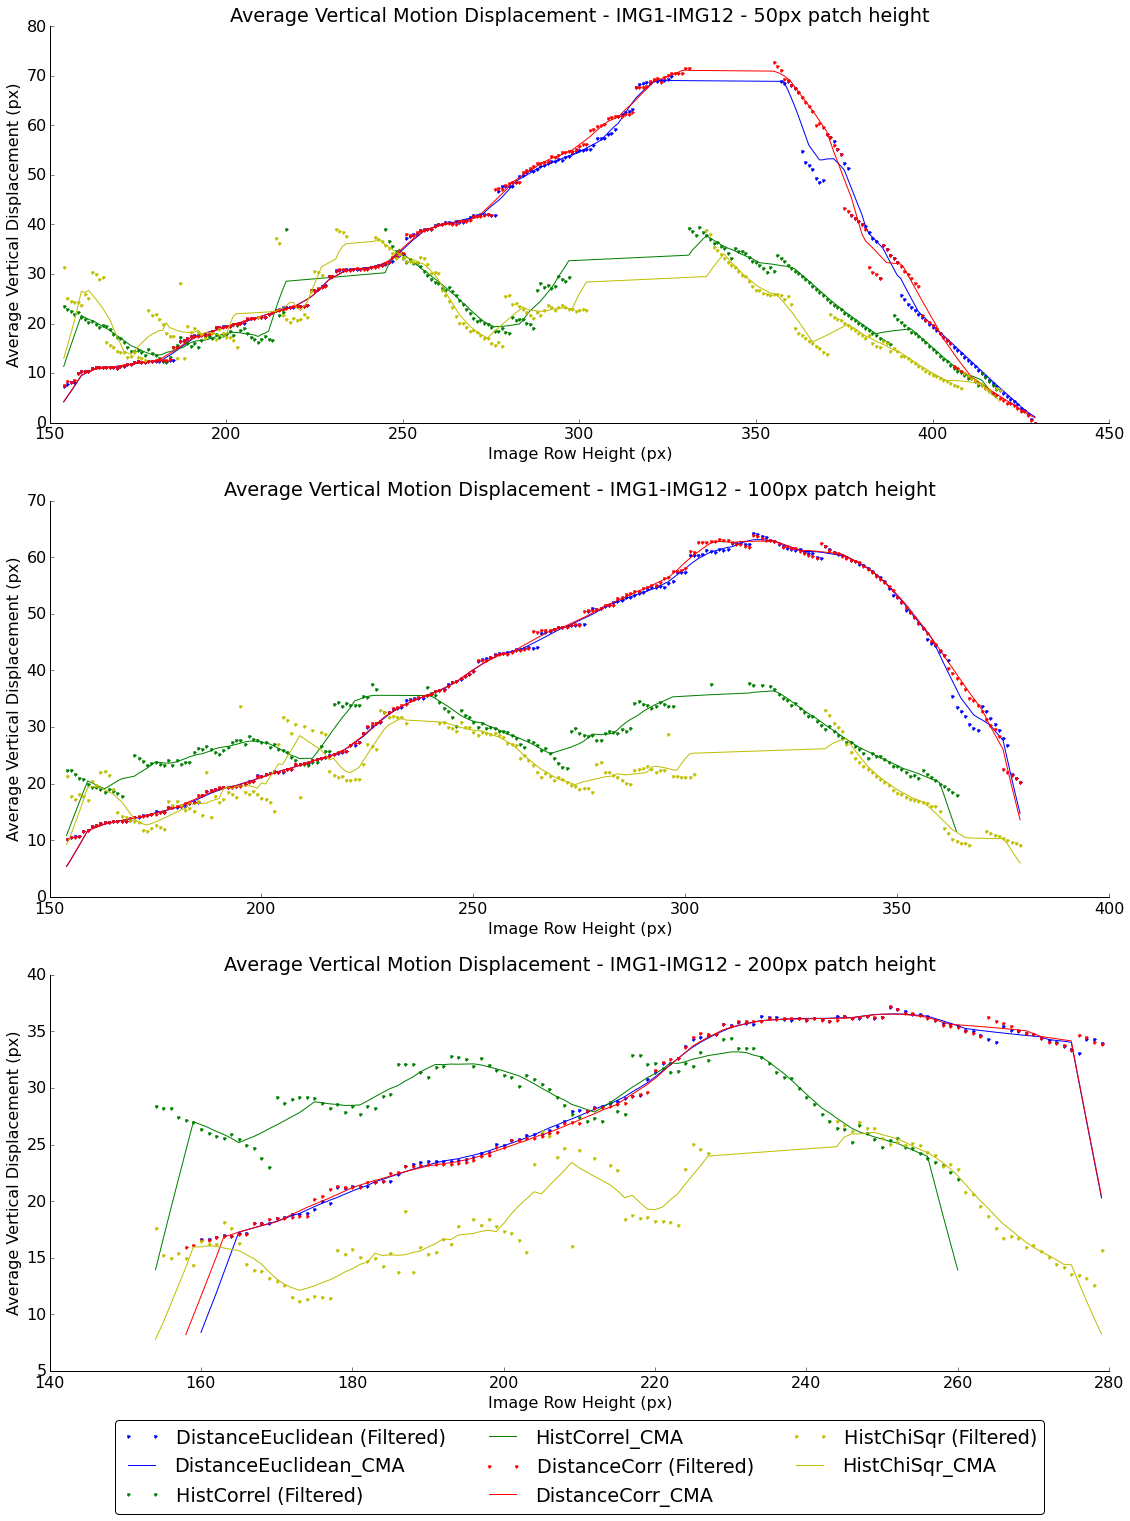
\includegraphics[scale=0.3]{images/results/flat_10cm_non_scaled_exhaustive}
\caption{Average vertical motion displacement models across all images within ``living room carpet" dataset running \textit{exhaustive} localised search. Graph 1 (Top) - Full-width patch with fixed height of 50px; Graph 2 (Middle) Full-width patch with fixed height of 100px; Graph 3 (Bottom) Full-width patch with fixed height of 200px. Solid line indicates centred moving average (10-pixel interval) calculated from filtered results for each appearance-based template matching similarity metric.}
\label{fig:ex2_1_2}
\end{figure}

Across the non-exhaustive, and exhaustive tests for dataset one (Figures \ref{fig:ex2_1_1} and \ref{fig:ex2_1_2} respectively) the two distance-based similarity measures provide clear examples of the expected positive relationship between the row within the image, and the level of vertical displacement. However, in the case of all three of the tested patch sizes, the results from the exhaustive search indicate a significantly smoother upwards trend than the non-exhaustive search.

\clearpage
\subsubsection{Dataset 2: Brick-Paved Road (Outside)}

\begin{figure}[ht!]
\centering
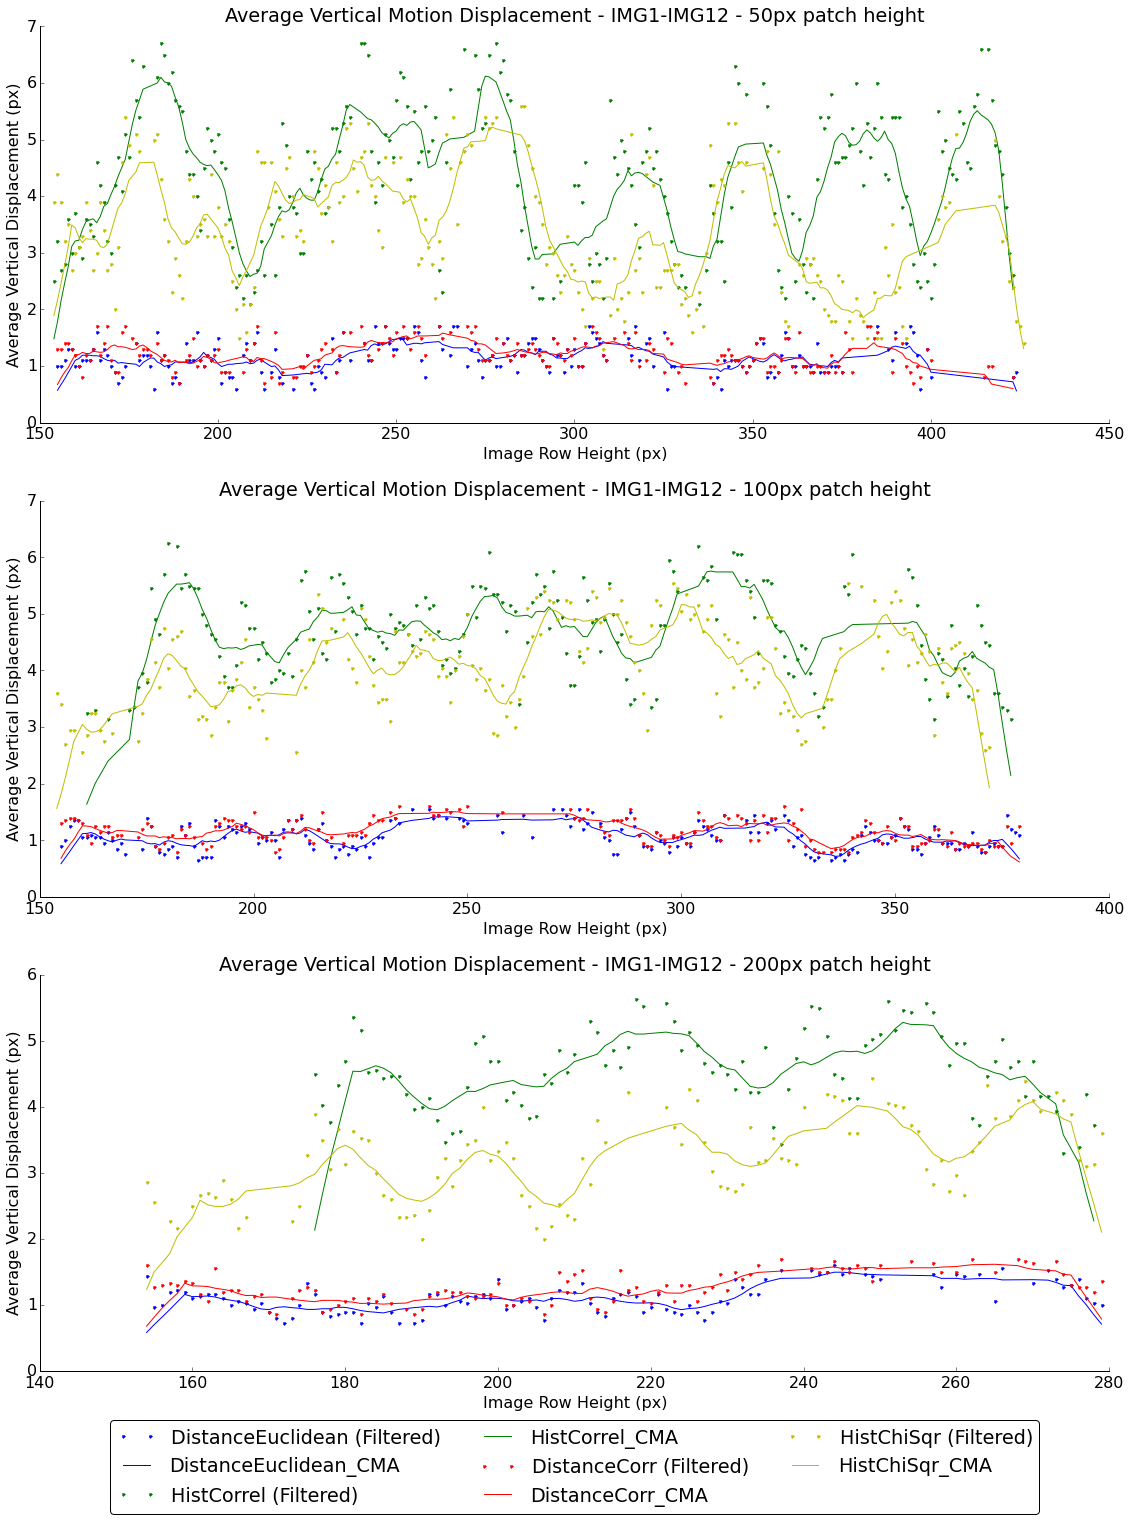
\includegraphics[scale=0.3]{images/results/wiltshire_outside_10cm_non_scaled}
\caption{Average vertical motion displacement models across all images within ``brick-paved drive" dataset running \textit{non-exhaustive} localised search. Graph 1 (Top) - Full-width patch with fixed height of 50px; Graph 2 (Middle) Full-width patch with fixed height of 100px; Graph 3 (Bottom) Full-width patch with fixed height of 200px. Solid line indicates centred moving average (10-pixel interval) calculated from filtered results for each appearance-based template matching similarity metric.}
\label{fig:ex2_2_1}
\end{figure}

\clearpage
\begin{figure}[ht!]
\centering
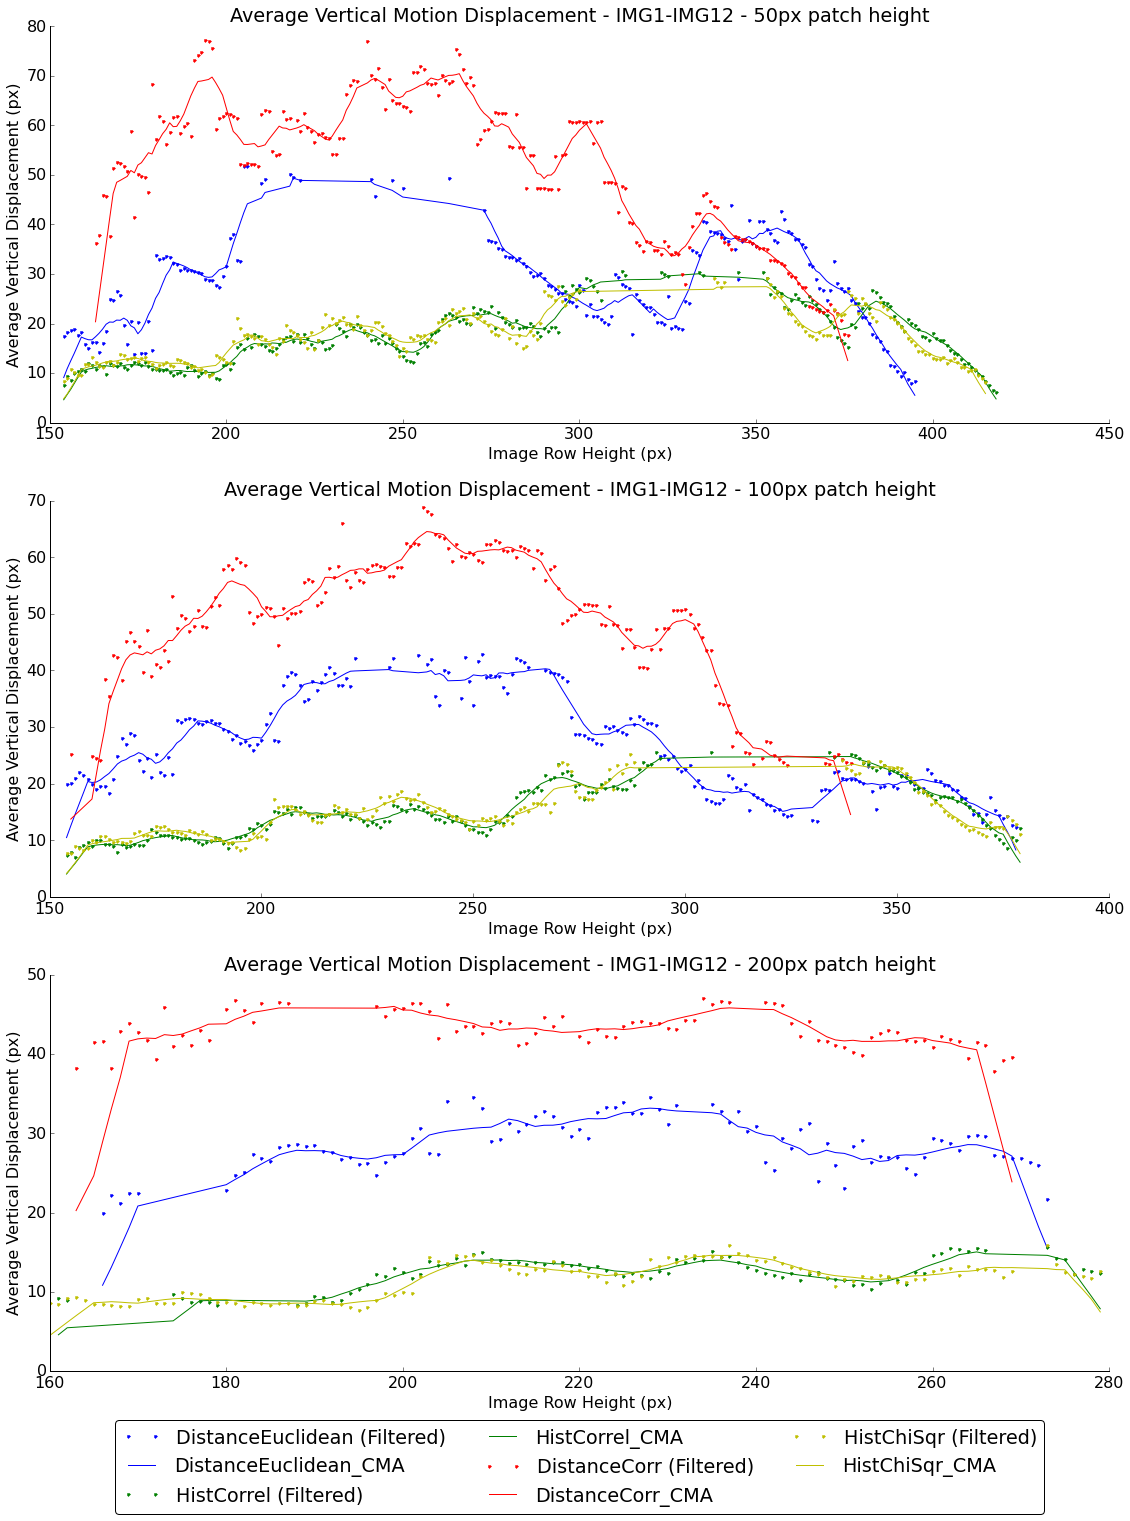
\includegraphics[scale=0.3]{images/results/wiltshire_outside_10cm_non_scaled_exhaustive}
\caption{Average vertical motion displacement models across all images within ``brick-paved drive" dataset running \textit{exhaustive} localised search. Graph 1 (Top) - Full-width patch with fixed height of 50px; Graph 2 (Middle) Full-width patch with fixed height of 100px; Graph 3 (Bottom) Full-width patch with fixed height of 200px. Solid line indicates centred moving average (10-pixel interval) calculated from filtered results for each appearance-based template matching similarity metric.}
\label{fig:ex2_2_2}
\end{figure}

The results recorded between the non-exhaustive, and exhaustive tests for dataset two (Figures \ref{fig:ex2_2_1} and \ref{fig:ex2_2_2} respectively) provide a stark contrast in performance between the two categories of similarity measure. Within the results of the non-exhaustive search, the two histogram-based measures indicate proportionally greater levels of displacement than the Normalised Cross-Correlation and Euclidean Distance measures. However this recorded displacement also demonstrates a considerable level of noise. In contrast, the results for the exhaustive search show greater levels of vertical displacement overall, but in this case it is the Euclidean Distance that provides the highest displacement, with Normalised Cross Correlation coming second.  

\clearpage
\subsubsection{Dataset 3: Asian Rug (Indoors)}

\begin{figure}[ht!]
\centering
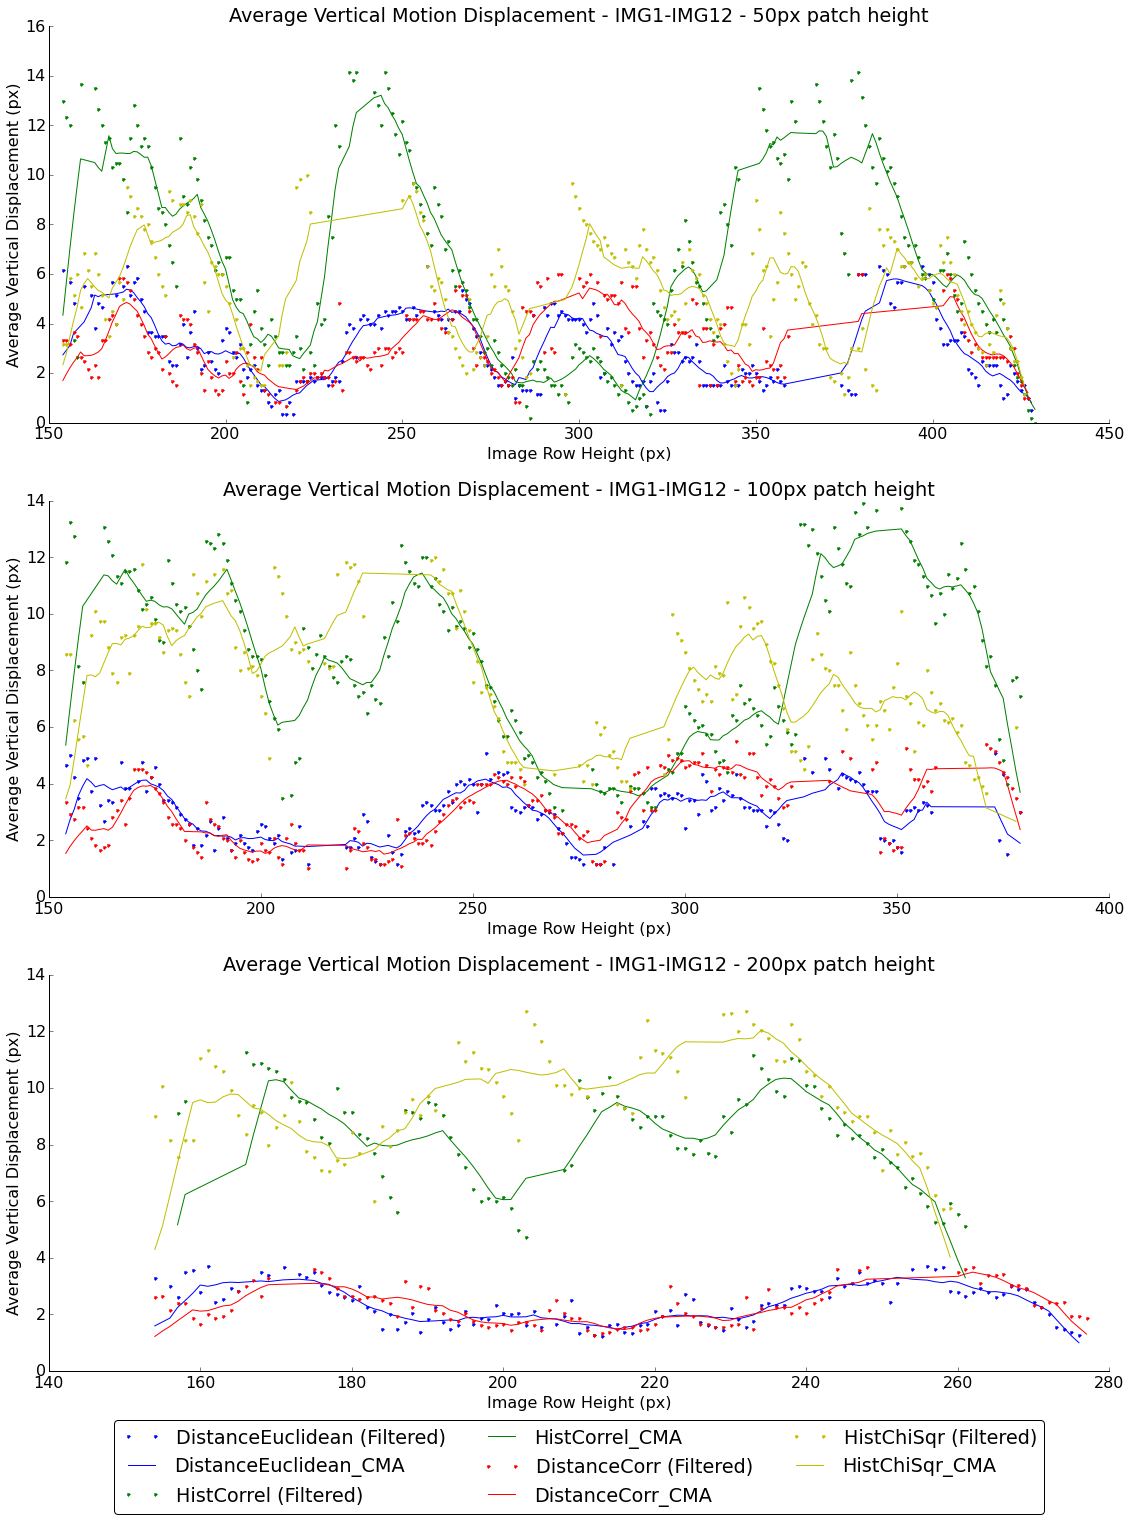
\includegraphics[scale=0.3]{images/results/wiltshire_inside_10cm_non_scaled}
\caption{Average vertical motion displacement models across all images within ``asian rug" dataset running \textit{non-exhaustive} localised search. Graph 1 (Top) - Full-width patch with fixed height of 50px; Graph 2 (Middle) Full-width patch with fixed height of 100px; Graph 3 (Bottom) Full-width patch with fixed height of 200px. Solid line indicates centred moving average (10-pixel interval) calculated from filtered results for each appearance-based template matching similarity metric.}
\label{fig:ex2_3_1}
\end{figure}

\clearpage
\begin{figure}[ht!]
\centering
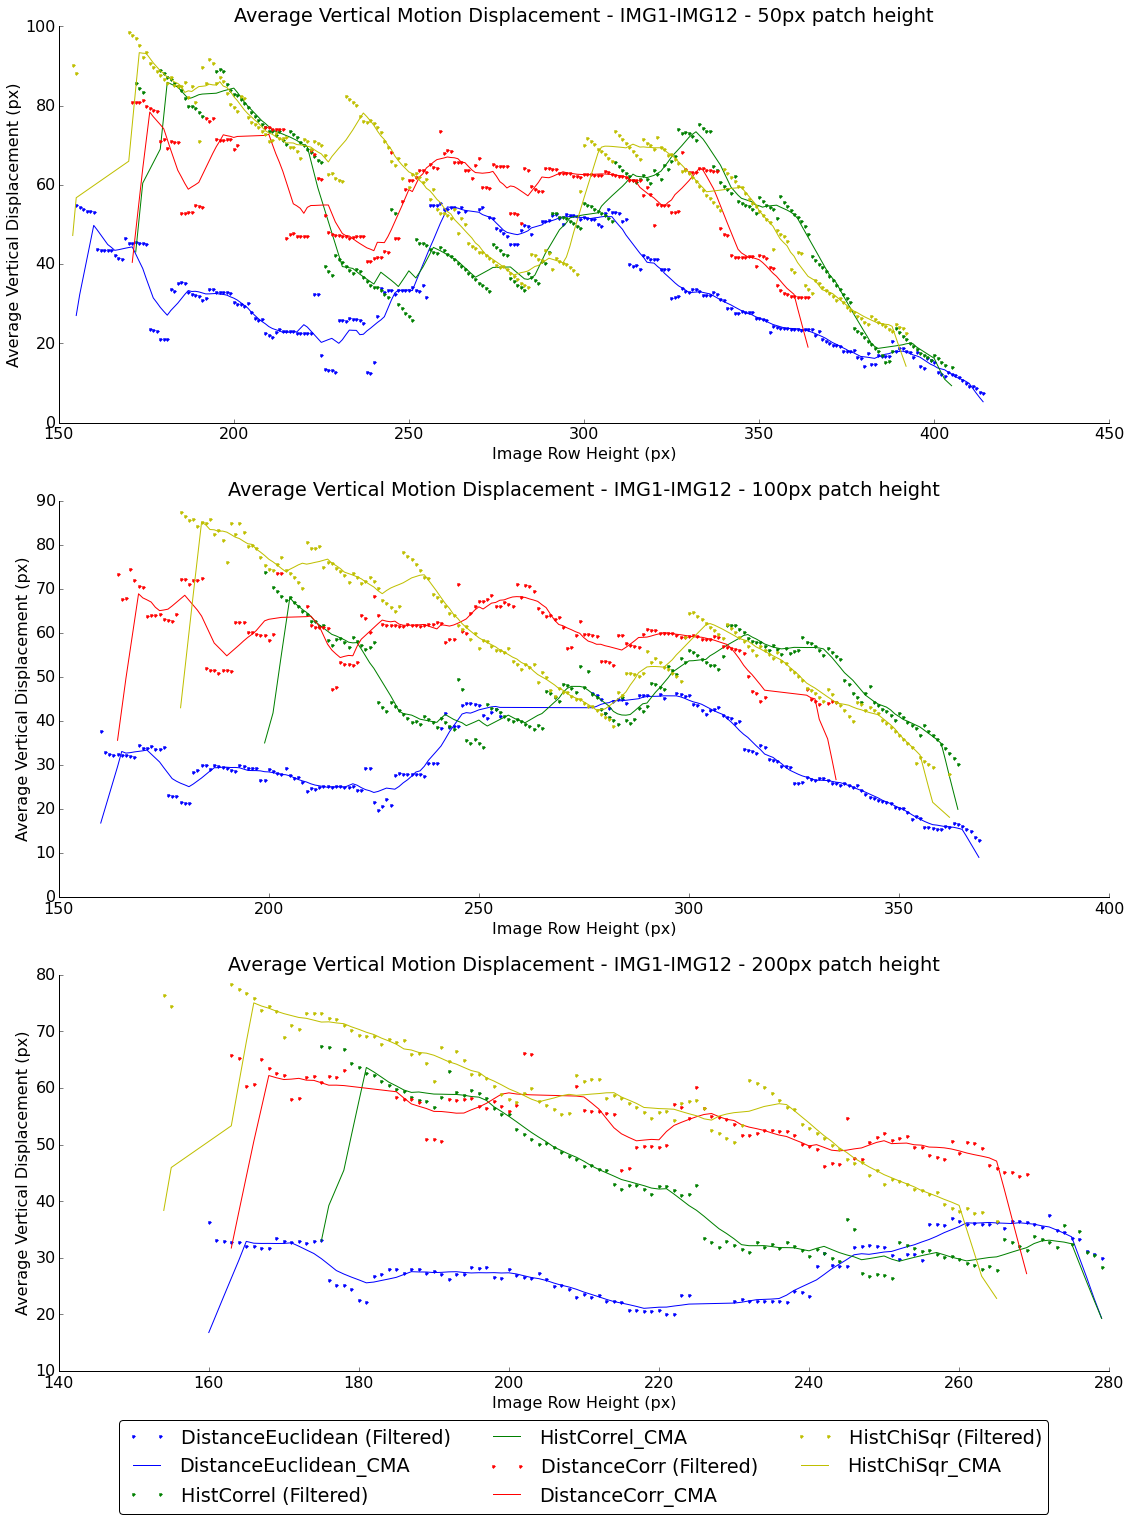
\includegraphics[scale=0.3]{images/results/wiltshire_inside_10cm_non_scaled_exhaustive}
\caption{Average vertical motion displacement models across all images within ``asian rug" dataset running \textit{exhaustive} localised search. Graph 1 (Top) - Full-width patch with fixed height of 50px; Graph 2 (Middle) Full-width patch with fixed height of 100px; Graph 3 (Bottom) Full-width patch with fixed height of 200px. Solid line indicates centred moving average (10-pixel interval) calculated from filtered results for each appearance-based template matching similarity metric.}
\label{fig:ex2_3_2}
\end{figure}

For dataset three, neither the exhaustive (Figure \ref{fig:ex2_3_1}), or non-exhaustive (Figure \ref{fig:ex2_3_2}) localised search approaches provide particularly desirable results, with all of the patch sizes and similarity measures demonstrating either just significant levels of noise with no correlation between image row and vertical displacement demonstrated, or in the case of the exhaustive search, less overall noise but a negative correlation, hence showing the opposite trend of what is expected. 

\clearpage
\subsubsection{Dataset 4: Slate Footpath (Outdoors)}

\begin{figure}[ht!]
\centering
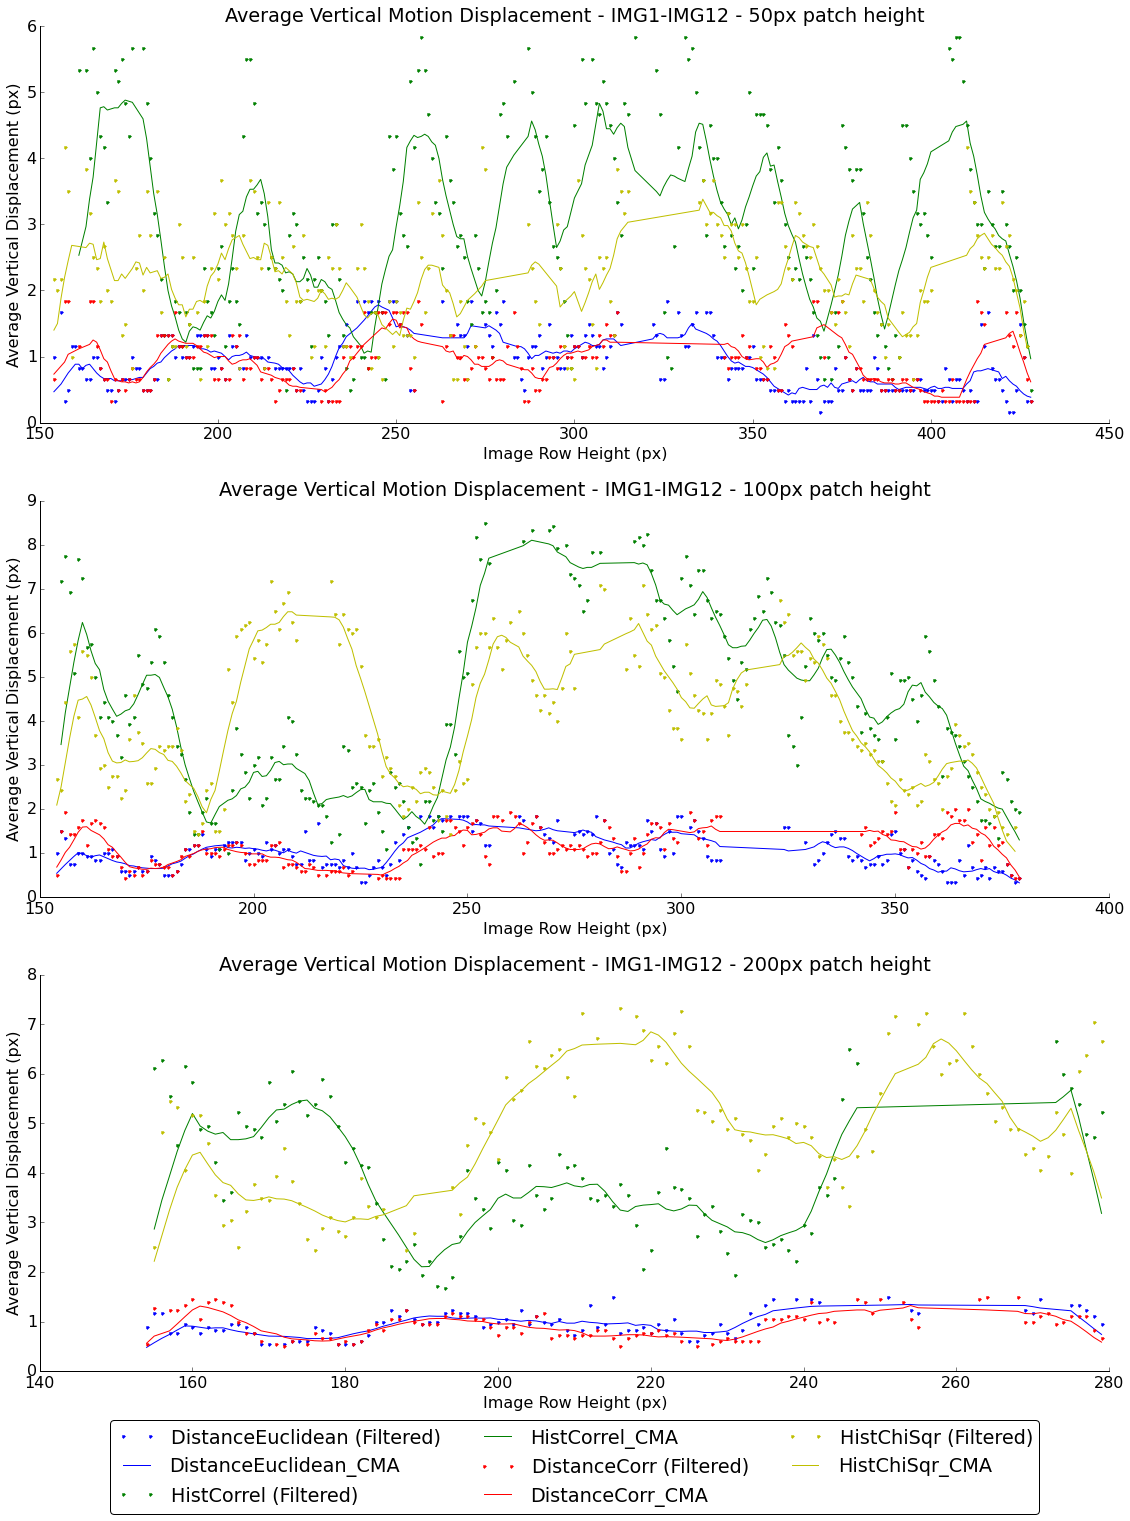
\includegraphics[scale=0.3]{images/results/path_outside_10cm_non_scaled}
\caption{Average vertical motion displacement models across all images within ``slate footpath" dataset running \textit{non-exhaustive} localised search. Graph 1 (Top) - Full-width patch with fixed height of 50px; Graph 2 (Middle) Full-width patch with fixed height of 100px; Graph 3 (Bottom) Full-width patch with fixed height of 200px. Solid line indicates centred moving average (10-pixel interval) calculated from filtered results for each appearance-based template matching similarity metric.}
\label{fig:ex2_4_1}
\end{figure}

\clearpage
\begin{figure}[ht!]
\centering
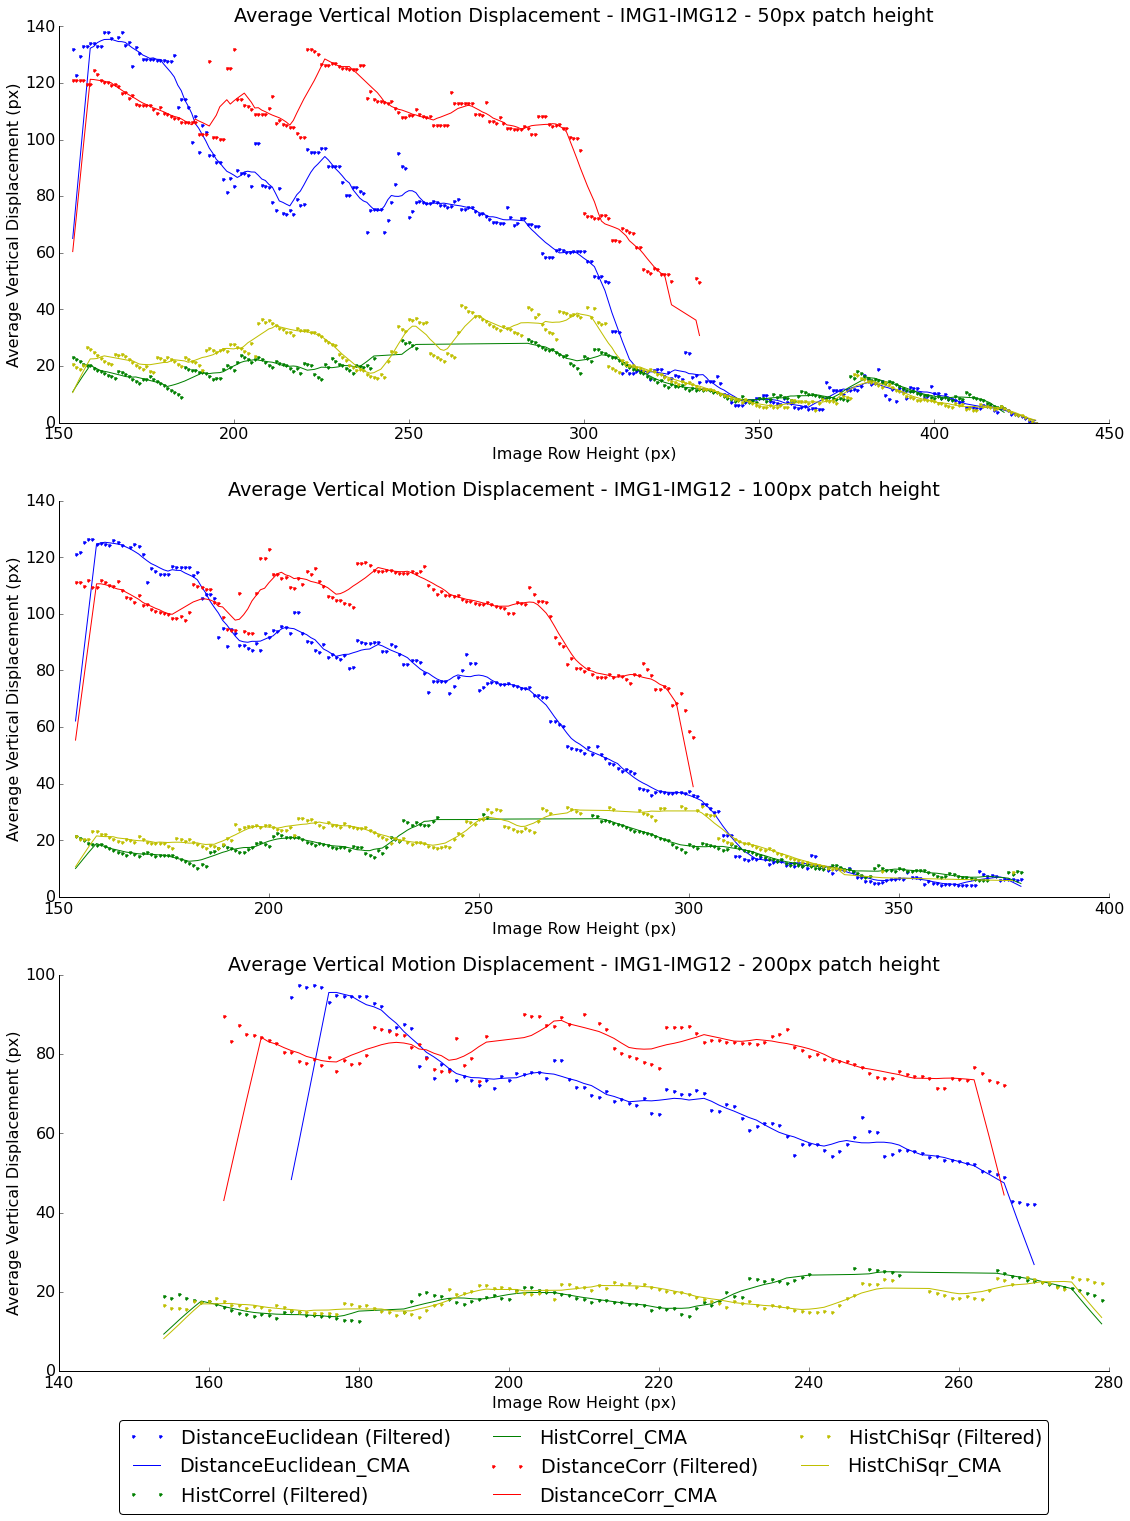
\includegraphics[scale=0.3]{images/results/path_outside_10cm_non_scaled_exhaustive}
\caption{Average vertical motion displacement models across all images within ``slate footpath" dataset running \textit{exhaustive} localised search. Graph 1 (Top) - Full-width patch with fixed height of 50px; Graph 2 (Middle) Full-width patch with fixed height of 100px; Graph 3 (Bottom) Full-width patch with fixed height of 200px. Solid line indicates centred moving average (10-pixel interval) calculated from filtered results for each appearance-based template matching similarity metric.}
\label{fig:ex2_4_2}
\end{figure}


The results for dataset four (Figures \ref{fig:ex2_4_1} and \ref{fig:ex2_4_2}) resemble those shown for the previous dataset (Figures \ref{fig:ex2_3_1} and \ref{fig:ex2_3_2}) whereby the non-exhaustive search results indicate high levels of noise and for exhaustive search results, while all patch sizes do indicate a definitive correlation between row height and the demonstrated vertical displacement, it is again a negative, rather than expected positive correlation. 

\clearpage
\subsection{Experiment 3: Template Matching (Full-width Patches - Scaled)}

\subsubsection{Dataset 1: Living Room Carpet (Indoors)}

\begin{figure}[ht!]
\centering
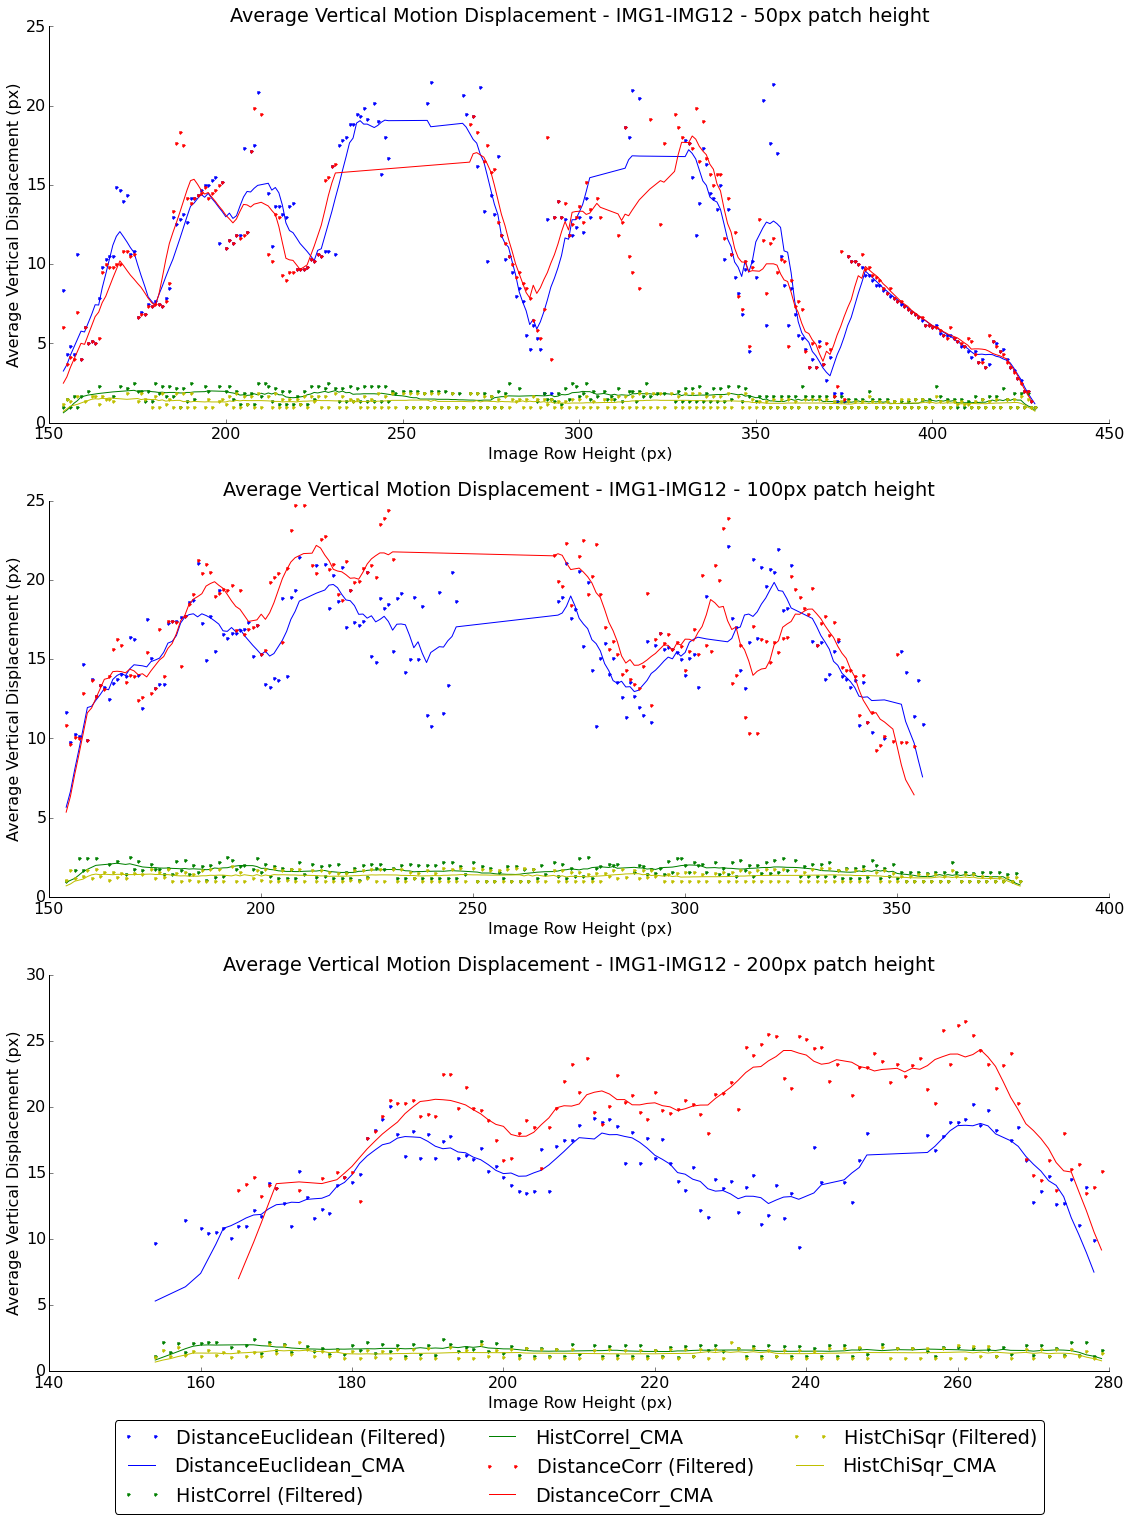
\includegraphics[scale=0.3]{images/results/flat_10cm_scaled}
\caption{Average vertical motion displacement models across all images within ``living room carpet" dataset running \textit{non-exhaustive} localised search with geometrically scaled template patches. Graph 1 (Top) - Full-width patch with fixed height of 50px; Graph 2 (Middle) Full-width patch with fixed height of 100px; Graph 3 (Bottom) Full-width patch with fixed height of 200px. Solid line indicates centred moving average (10-pixel interval) calculated from filtered results for each appearance-based template matching similarity metric.}
\label{fig:ex3_1_1}
\end{figure}

\clearpage
\begin{figure}[ht!]
\centering
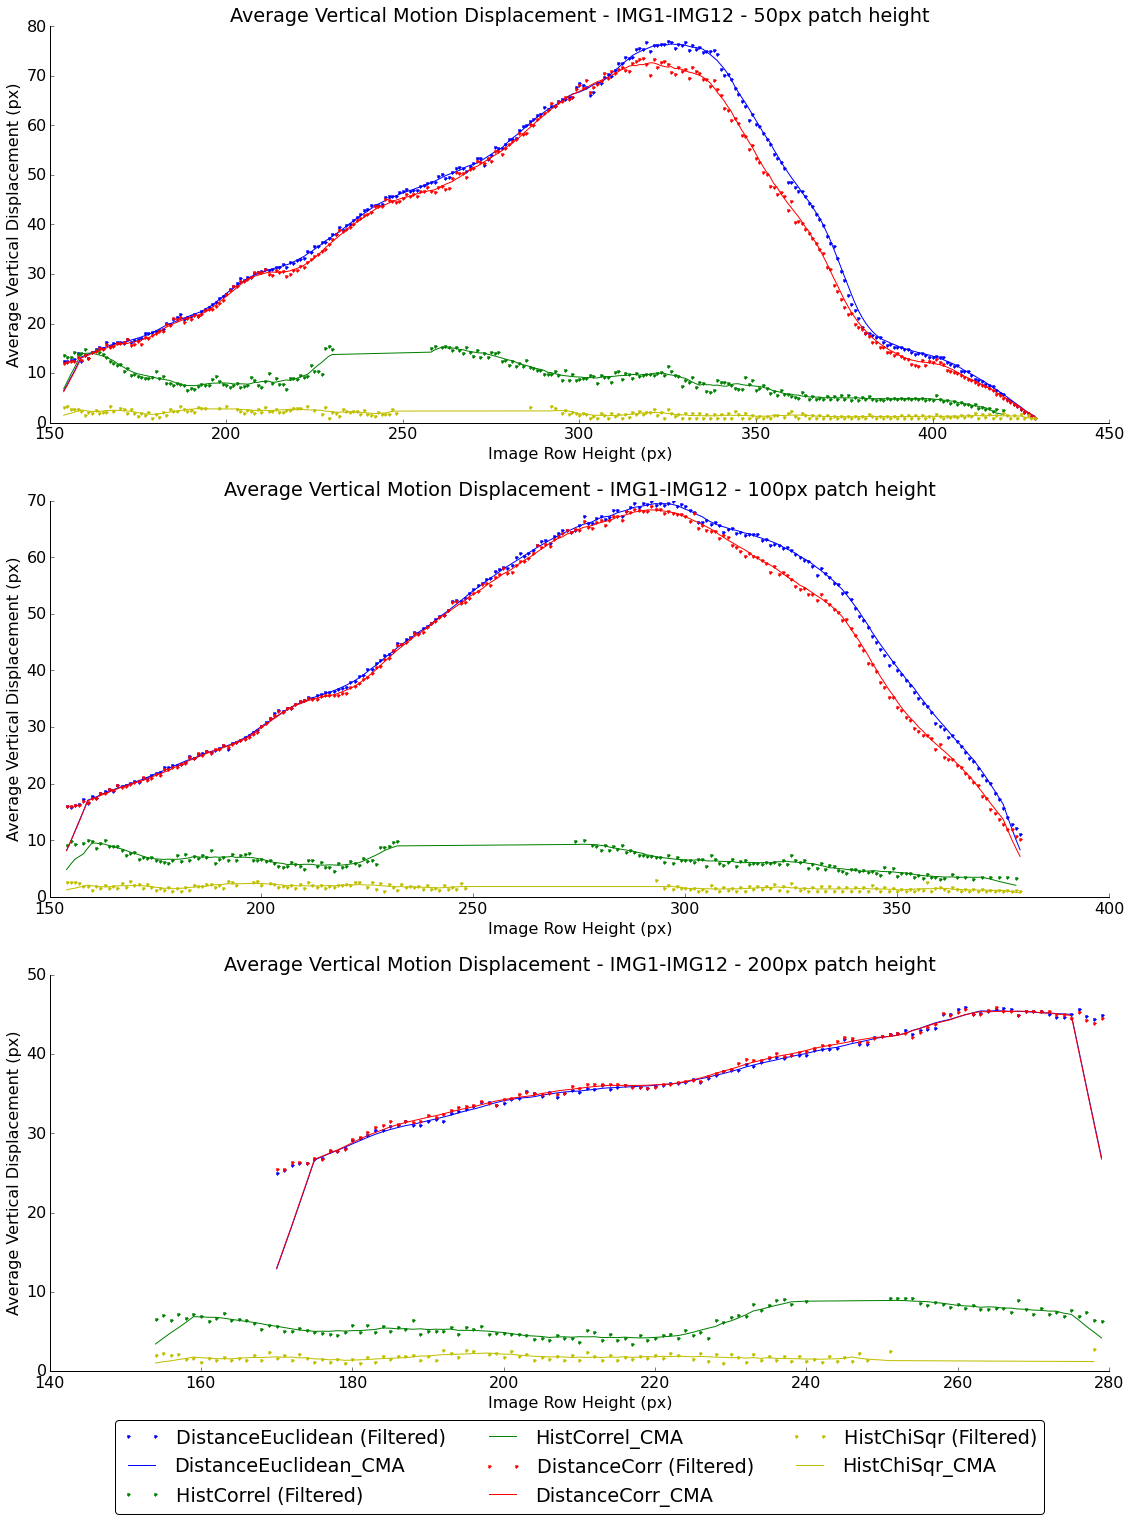
\includegraphics[scale=0.3]{images/results/flat_10cm_scaled_exhaustive}
\caption{Average vertical motion displacement models across all images within ``living room carpet" dataset running \textit{exhaustive} localised search with geometrically scaled template patches. Graph 1 (Top) - Full-width patch with fixed height of 50px; Graph 2 (Middle) Full-width patch with fixed height of 100px; Graph 3 (Bottom) Full-width patch with fixed height of 200px. Solid line indicates centred moving average (10-pixel interval) calculated from filtered results for each appearance-based template matching similarity metric.}
\label{fig:ex3_1_2}
\end{figure}

The results for dataset one appear to indicate a difference between the performance of the non-exhaustive search (Figure \ref{fig:ex3_1_1}) vs the exhaustive search (Figure \ref{fig:ex3_1_2}) when performing scaling of the template patch. Within the non-exhaustive results, while the third test using the 200px-height patch (Fig: \ref{fig:ex3_1_1} Graph 3) does appear to show the expected positive correlation, the tests involving the smaller patches are more susceptible to noise (with the smallest patch showing the most distortion). In contrast to this, all three of the exhaustive searches demonstrate a strong and well defined positive correlation for both of the distance-based similarity measures. For all tests performed on dataset one,the histogram-based approaches to record any significant displacement fails.

\clearpage
\subsubsection{Dataset 2: Brick-Paved Road (Outside)}

\begin{figure}[ht!]
\centering
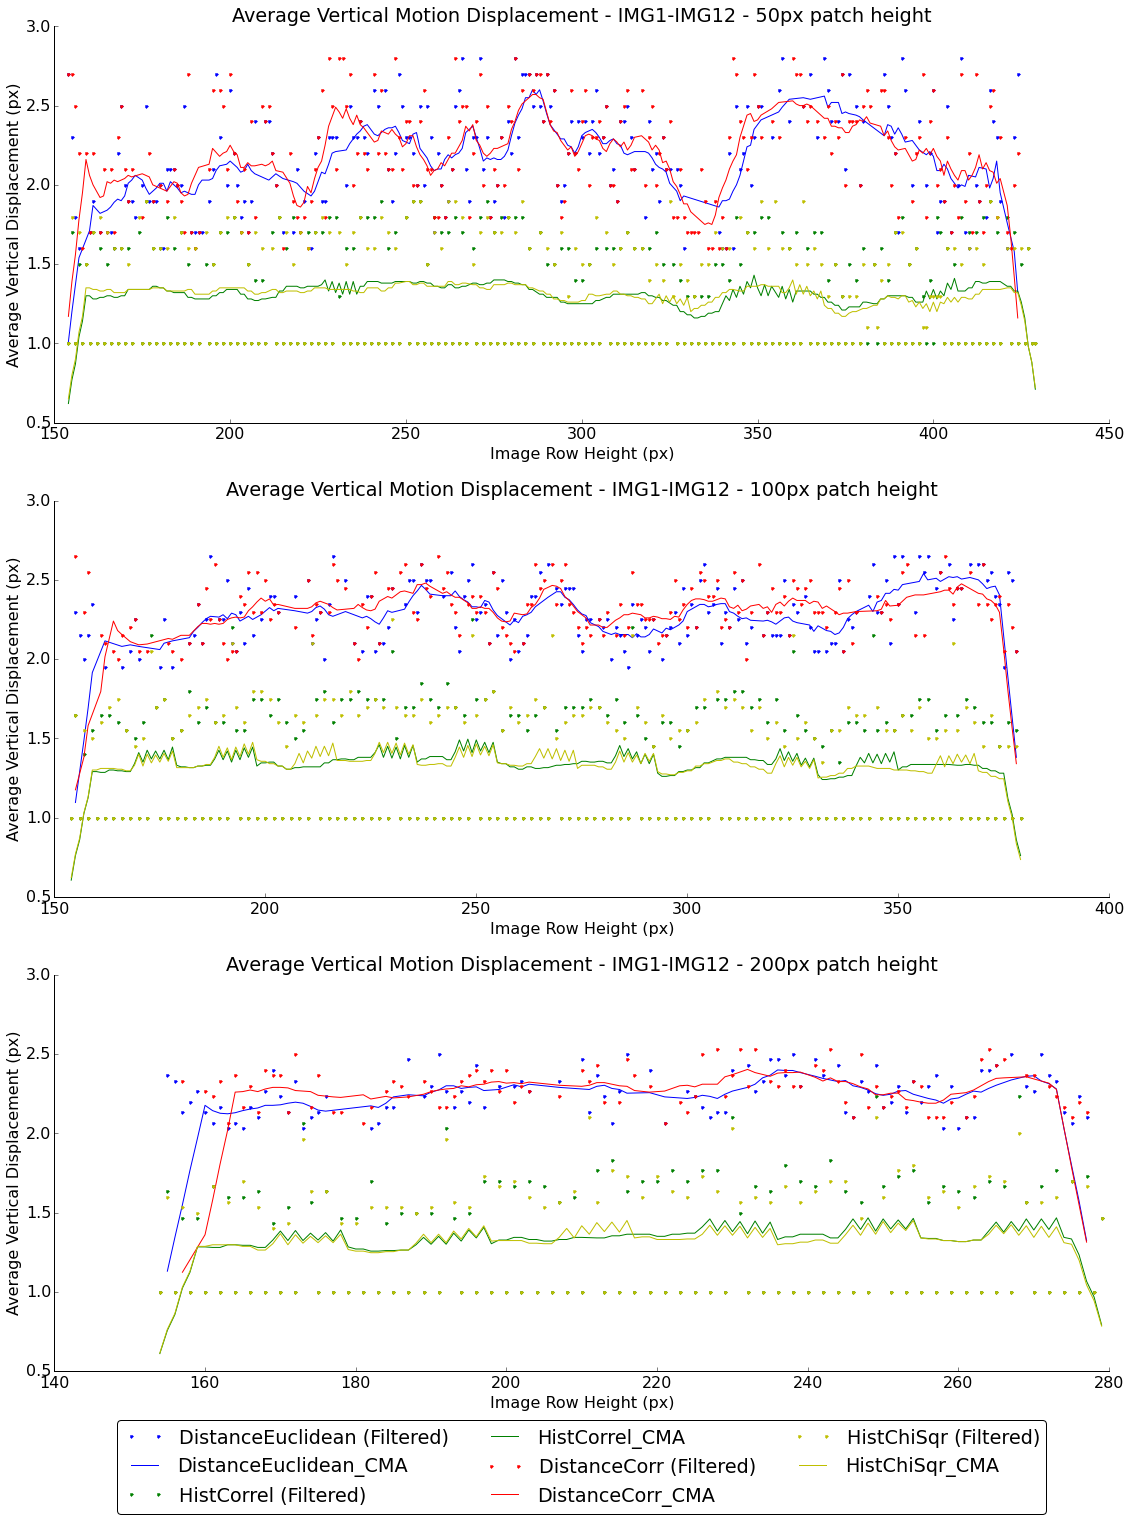
\includegraphics[scale=0.3]{images/results/wiltshire_outside_10cm_scaled}
\caption{Average vertical motion displacement models across all images within ``brick-paved drive" dataset running \textit{non-exhaustive} localised search with geometrically scaled template patches. Graph 1 (Top) - Full-width patch with fixed height of 50px; Graph 2 (Middle) Full-width patch with fixed height of 100px; Graph 3 (Bottom) Full-width patch with fixed height of 200px. Solid line indicates centred moving average (10-pixel interval) calculated from filtered results for each appearance-based template matching similarity metric.}
\label{fig:ex3_2_1}
\end{figure}

\clearpage
\begin{figure}[ht!]
\centering
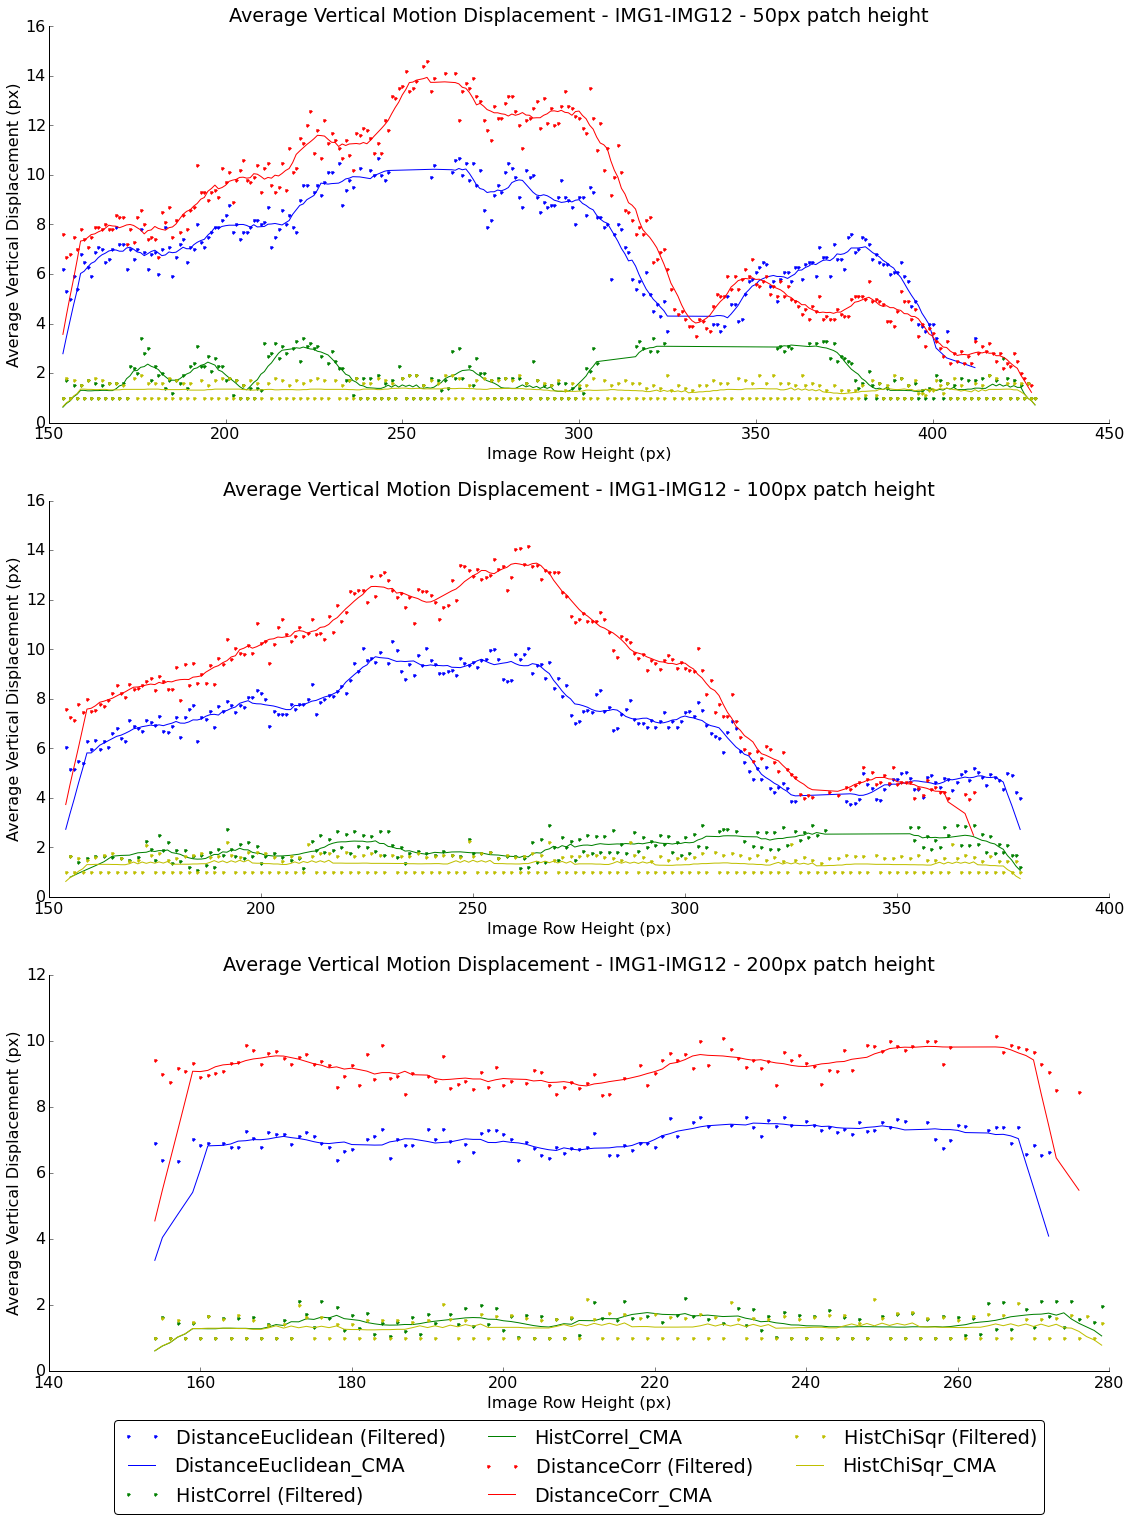
\includegraphics[scale=0.3]{images/results/wiltshire_outside_10cm_scaled_exhaustive}
\caption{Average vertical motion displacement models across all images within ``brick-paved drive" dataset running \textit{exhaustive} localised search with geometrically scaled template patches. Graph 1 (Top) - Full-width patch with fixed height of 50px; Graph 2 (Middle) Full-width patch with fixed height of 100px; Graph 3 (Bottom) Full-width patch with fixed height of 200px. Solid line indicates centred moving average (10-pixel interval) calculated from filtered results for each appearance-based template matching similarity metric.}
\label{fig:ex3_2_2}
\end{figure}

Under the non-exhaustive tests for dataset two (Figure \ref{fig:ex3_2_1}), all four similarity measures appear to indicate an approximately equal level of vertical displacement regardless of the row height, with a small maximum displacement measured (approx. 2-3px). Interestingly, this similar behaviour between the four similarity metrics is demonstrated across all three patches (although the level of noise demonstrated does decrease as the patch size increases). For the exhaustive search (Figure \ref{fig:ex3_2_2}), a general positive correlation does begin to emerge for 50px and 100px patch heights under the distance-based similarity measures, however the results for the 200px patch size appear to show a lack of correlation, in the same way as for the corresponding test within the non-exhaustive results (Fig \ref{fig:ex3_2_1} Chart 3). 

\clearpage
\subsubsection{Dataset 3: Asian Rug (Indoors)}

\begin{figure}[ht!]
\centering
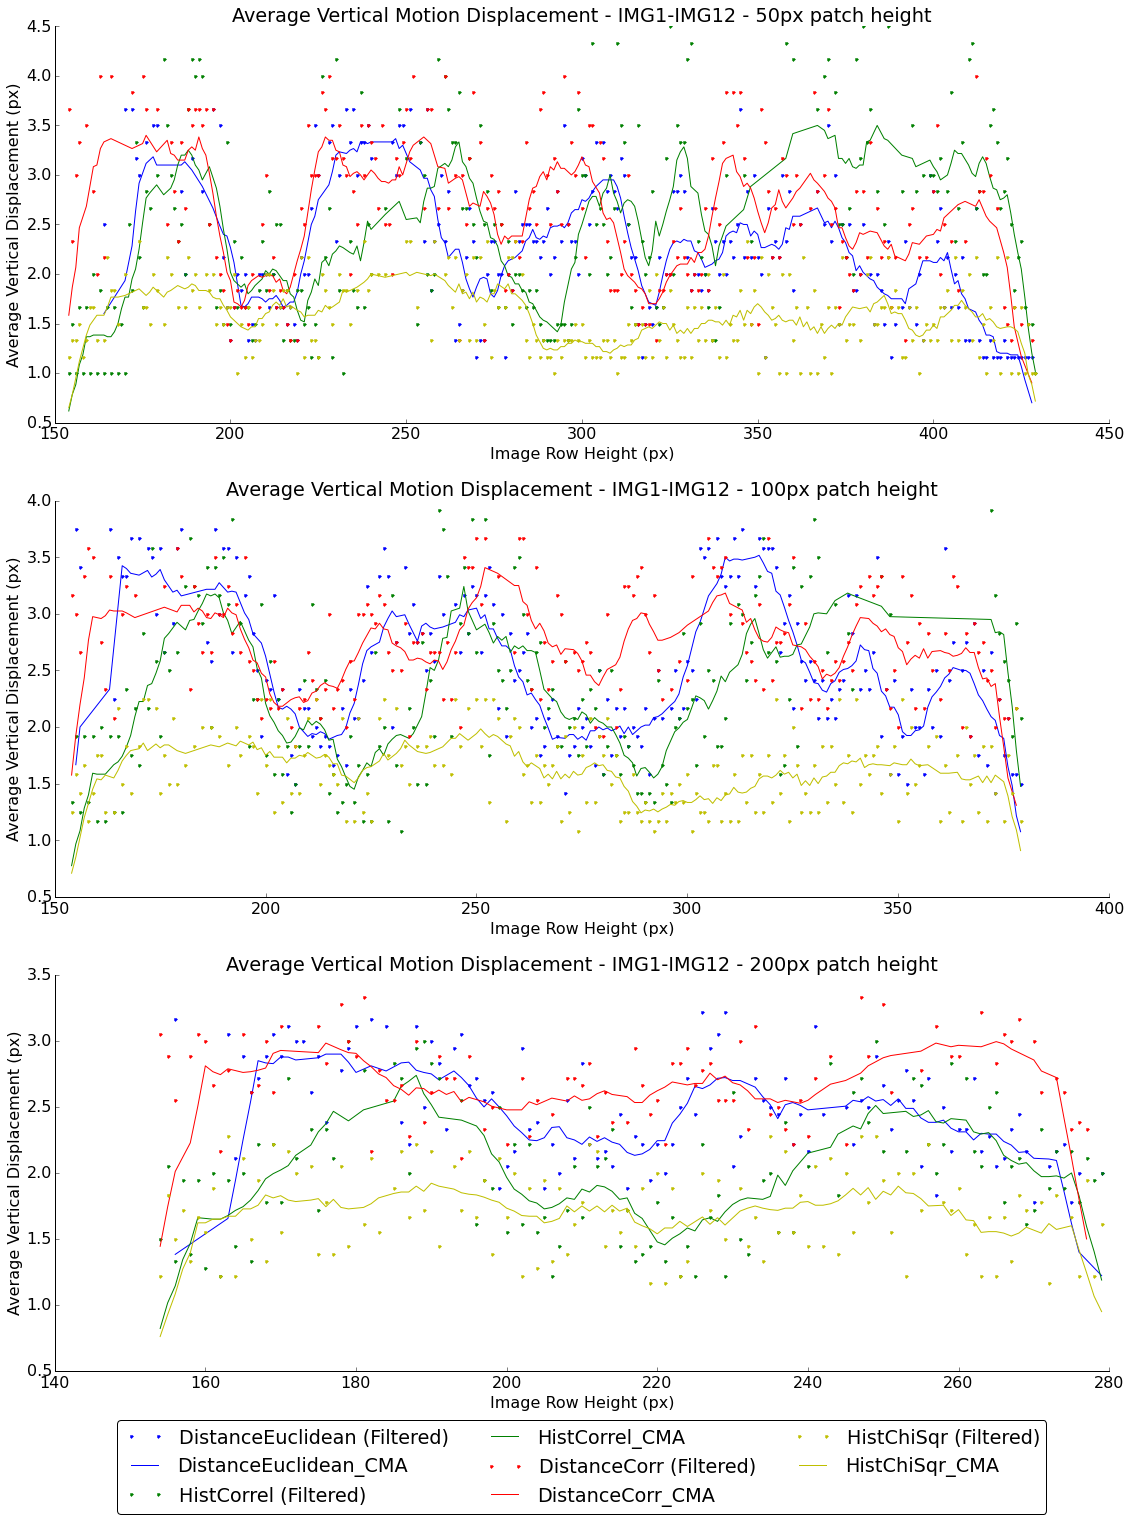
\includegraphics[scale=0.3]{images/results/wiltshire_inside_10cm_scaled}
\caption{Average vertical motion displacement models across all images within ``asian rug" dataset running \textit{non-exhaustive} localised searchwith geometrically scaled template patches. Graph 1 (Top) - Full-width patch with fixed height of 50px; Graph 2 (Middle) Full-width patch with fixed height of 100px; Graph 3 (Bottom) Full-width patch with fixed height of 200px. Solid line indicates centred moving average (10-pixel interval) calculated from filtered results for each appearance-based template matching similarity metric.}
\label{fig:ex3_3_1}
\end{figure}

\clearpage
\begin{figure}[ht!]
\centering
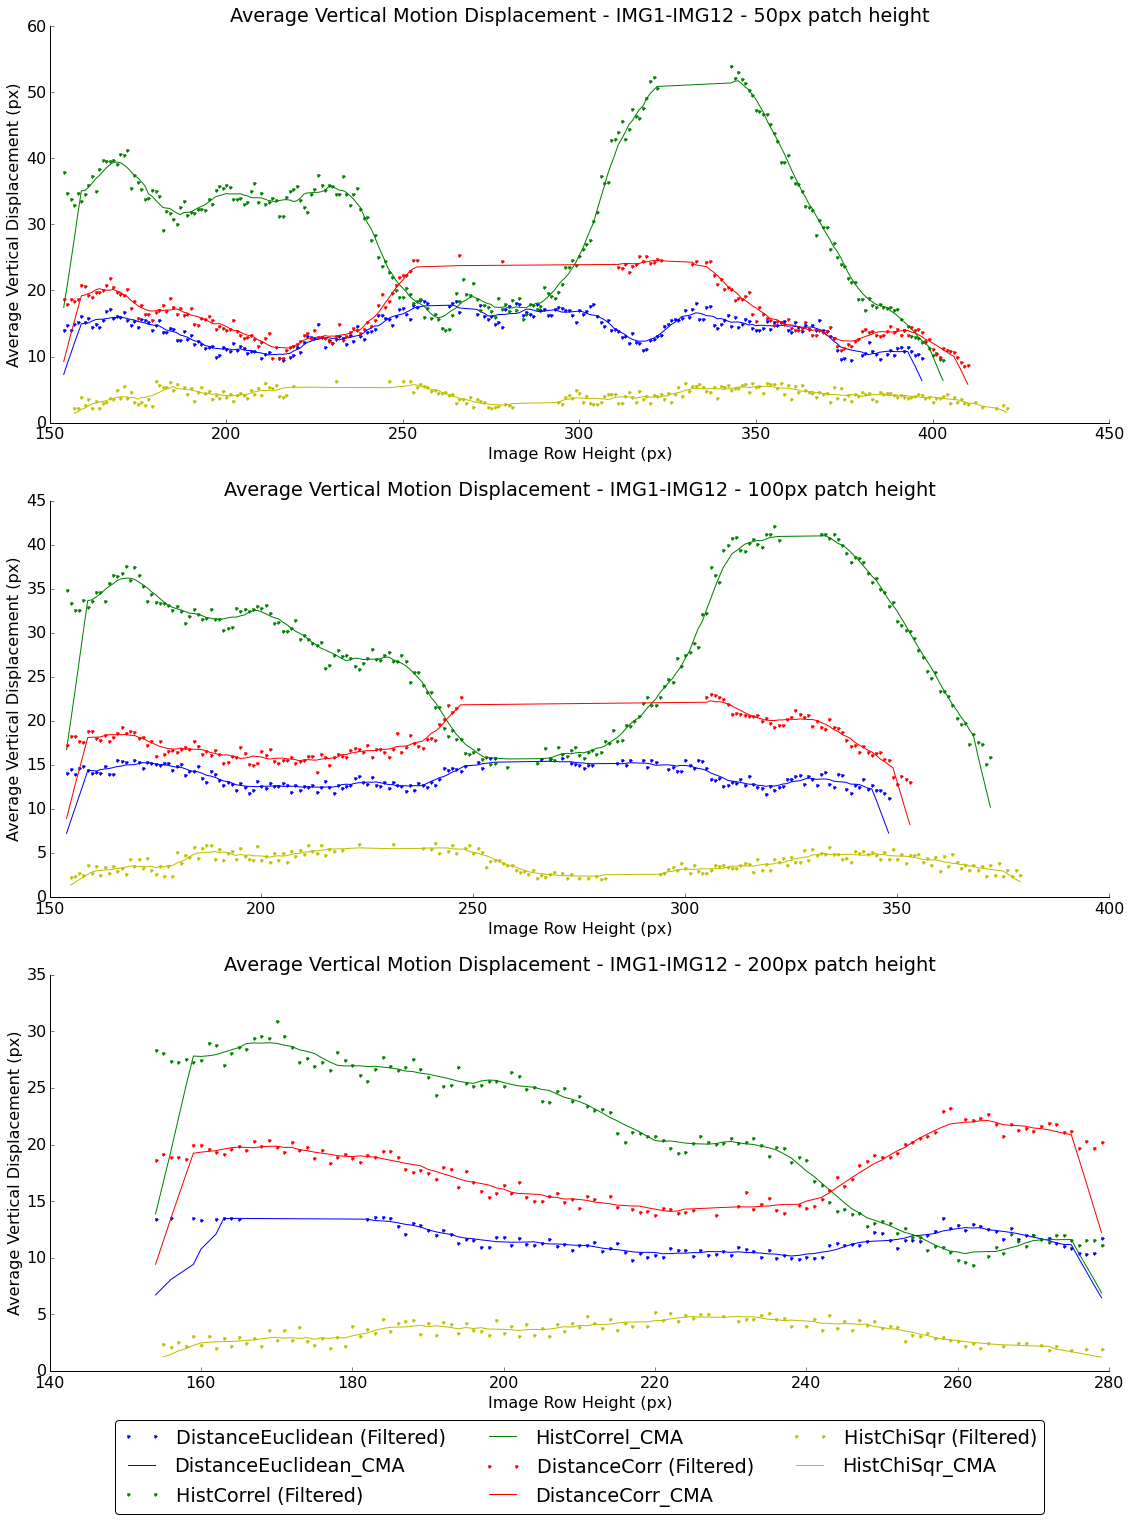
\includegraphics[scale=0.3]{images/results/wiltshire_inside_10cm_scaled_exhaustive}
\caption{Average vertical motion displacement models across all images within ``asian rug" dataset running \textit{exhaustive} localised search with geometrically scaled template patches. Graph 1 (Top) - Full-width patch with fixed height of 50px; Graph 2 (Middle) Full-width patch with fixed height of 100px; Graph 3 (Bottom) Full-width patch with fixed height of 200px. Solid line indicates centred moving average (10-pixel interval) calculated from filtered results for each appearance-based template matching similarity metric.}
\label{fig:ex3_3_2}
\end{figure}

As observed in the experiment two results for dataset three (Figure \ref{fig:ex2_3_1}), the non-exhaustive search (Figure \ref{fig:ex3_3_1}) appear to consist predominantly of noise, and with no correlation. Within the exhaustive search results (Figure \ref{fig:ex3_3_2}), the different categories of similarity measure appear to at times, demonstrate opposite correlation behaviours. In the particular case of the 200px patch-height test (Graph 3), the histogram-based Correlation metric shows an overall negative correlation, while the two distance-based metrics demonstrate a weak positive correlation.

\clearpage
\subsubsection{Dataset 4: Slate Footpath (Outdoors)}

\begin{figure}[ht!]
\centering
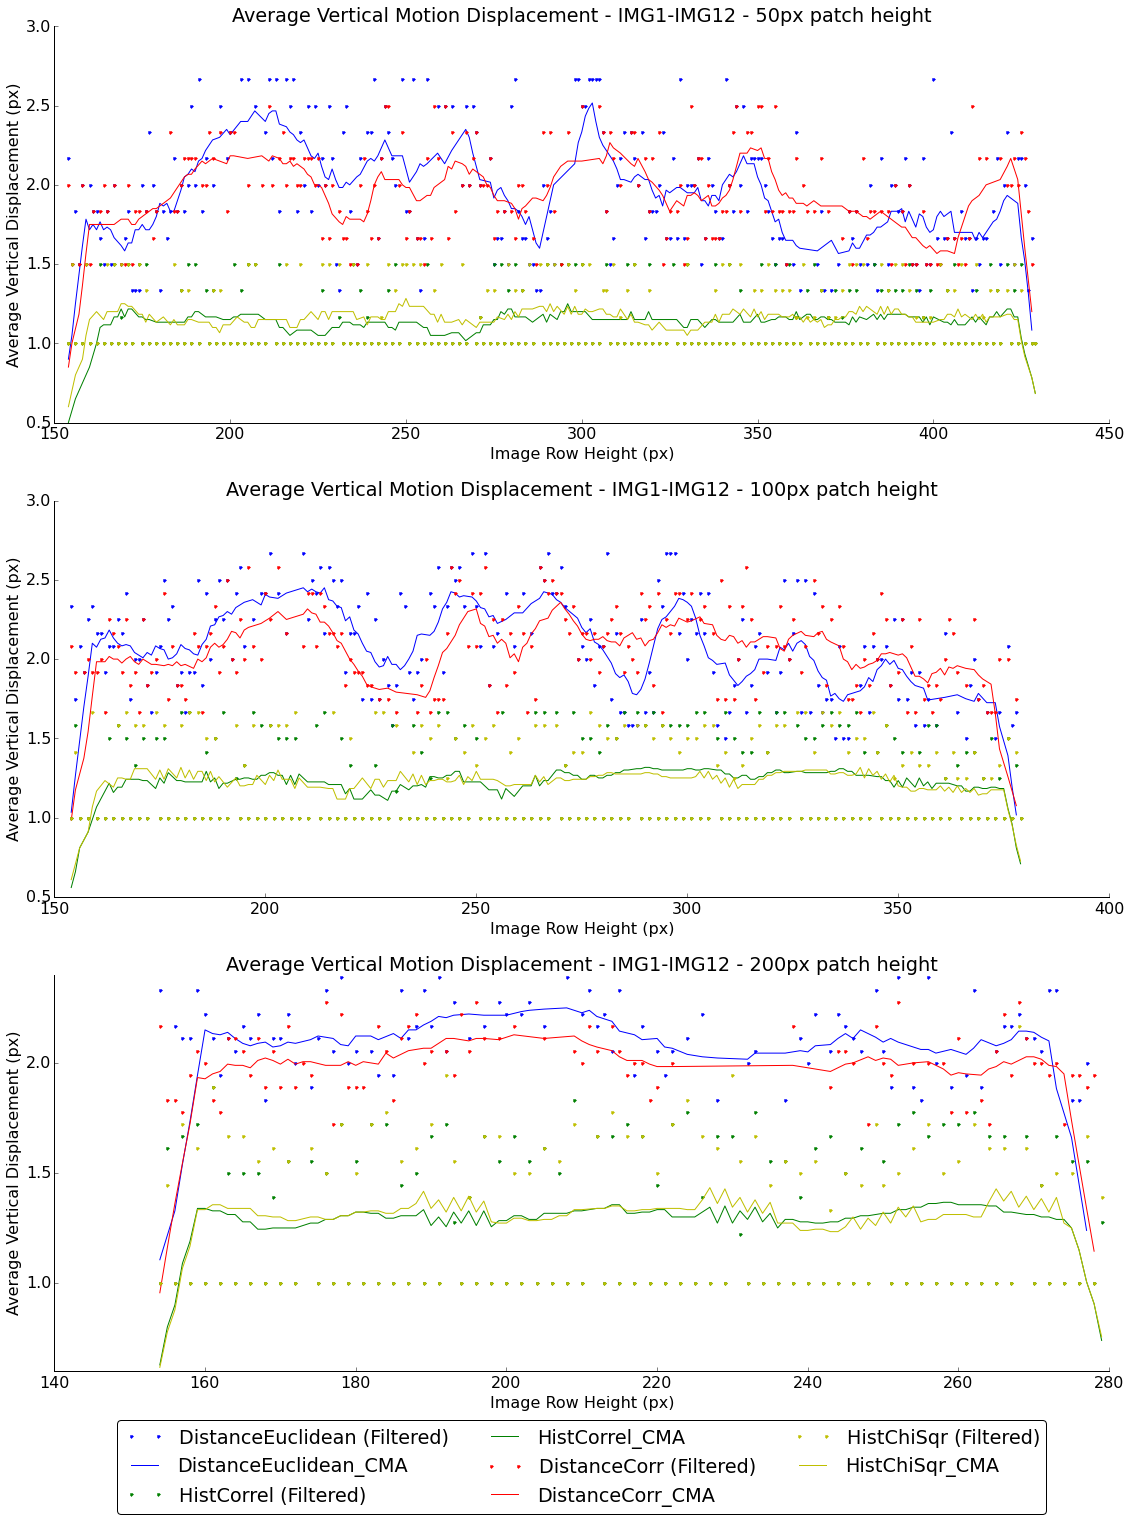
\includegraphics[scale=0.3]{images/results/path_outside_10cm_scaled}
\caption{Average vertical motion displacement models across all images within ``slate footpath" dataset running \textit{non-exhaustive} localised search with geometrically scaled template patches. Graph 1 (Top) - Full-width patch with fixed height of 50px; Graph 2 (Middle) Full-width patch with fixed height of 100px; Graph 3 (Bottom) Full-width patch with fixed height of 200px. Solid line indicates centred moving average (10-pixel interval) calculated from filtered results for each appearance-based template matching similarity metric.}
\label{fig:ex3_4_1}
\end{figure}

\clearpage
\begin{figure}[ht!]
\centering
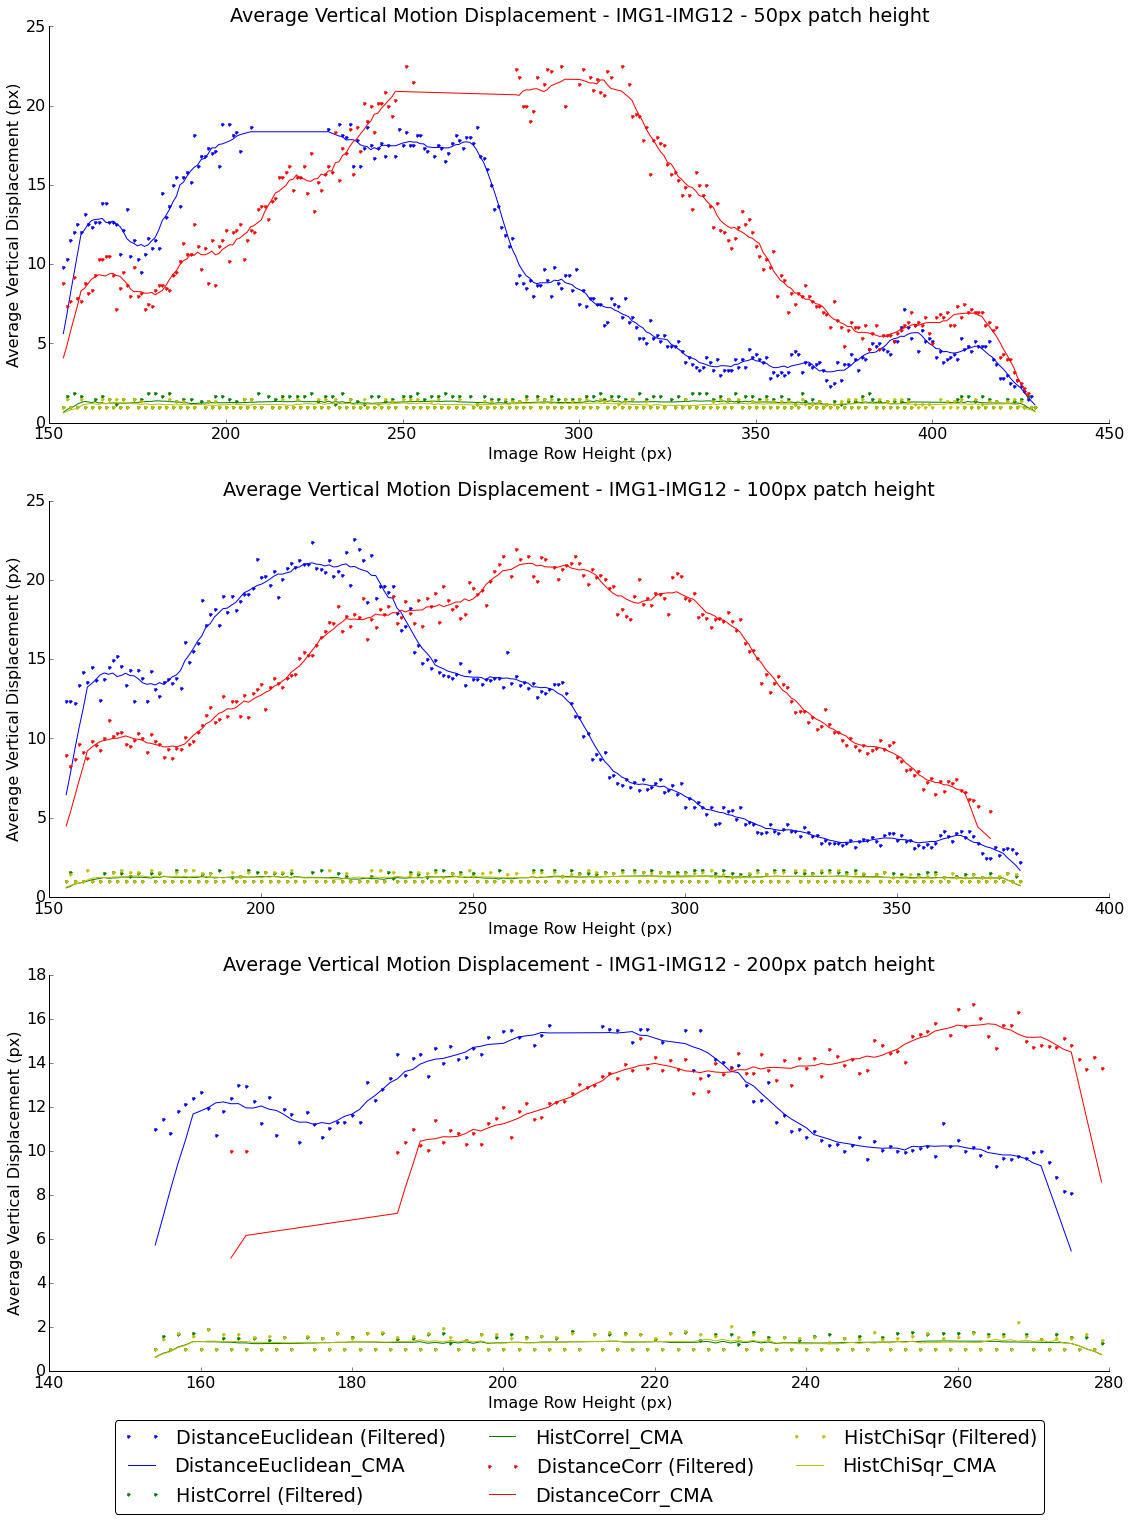
\includegraphics[scale=0.3]{images/results/path_outside_10cm_scaled_exhaustive}
\caption{Average vertical motion displacement models across all images within ``slate footpath" dataset running \textit{exhaustive} localised search with geometrically scaled template patches. Graph 1 (Top) - Full-width patch with fixed height of 50px; Graph 2 (Middle) Full-width patch with fixed height of 100px; Graph 3 (Bottom) Full-width patch with fixed height of 200px. Solid line indicates centred moving average (10-pixel interval) calculated from filtered results for each appearance-based template matching similarity metric.}
\label{fig:ex3_4_2}
\end{figure}

The results for dataset four show that for the non-exhaustive tests (Figure \ref{fig:ex3_4_1}), all of the similarity measures demonstrate significant of levels of noise, with the two distance-based metrics showing a greater level of variability in the results than the two histogram-based metrics. Within the exhaustive results (Figure \ref{fig:ex3_4_2}), a clear performance difference between the two categories of similarity measure is apparent, with the Normalised Cross-Correlation metric showing better overall correlation behaviour than the Euclidean Distance.


\clearpage
\section{Discussion of Results}

Across all three experiments and within all four datasets tested, the results obtained appear to be mixed in terms of the producing the expected performance, however the relative successes and failures of each experiment can be decomposed into a number of different aspects.

\subsection{Fixed Dimension of Patches}

The first of these aspects to consider is the variety of patch sizes, these have remained consistent for each experiment and dataset. 

In terms of robustness to noise, it was the 200px patch size that demonstrated the best overall resilience, in its results caused by erratic matching of incorrect corresponding patches. This is particularly visible in Figures \ref{fig:ex3_4_1}, \ref{fig:ex2_2_2} and \ref{fig:ex2_3_2}, where it is possible to observe a clear smoothing of the results between the 50px and 100px patch sizes, and those of the 200px patch size. Overall it is the 50px patch size that demonstrates the greatest level of noise in results across all experiments. This is most likely caused by the patch size being too small, resulting in the patch failing to extract a large enough region within the image from which it is possible to identify at least one unique feature that can be used to subsequently locate the same unique feature within the second image. At a patch size of 100px, the results obtained indicate a general level of noise that falls between the two extremities observed in the 50px and 200px patch sizes. 

While the results for the 200px patch size may be less prone to noise, they do also indicate a lack of sensitivity to observed vertical displacement. As can be seen in Figures \ref{fig:ex2_2_1}, \ref{fig:ex2_2_2}, \ref{fig:ex3_2_1}, \ref{fig:ex3_2_2} and \ref{fig:ex3_4_1}, while a level of vertical displacement continues to be recorded for the 200px patch size (Graph 3), when compared to the 50px and 100px patch sizes, the level of recorded displacement appears to remain almost constant across all rows within the image. This behaviour would not be expected, and does appear to be isolated to the use of the 200px patch size. The most likely cause is the patch size extracts a template region covering too large an area of the image scene, resulting in little variability of displacement being identified on account of the images only ever showing a relatively small level of motion change between each other. 

It should be noted that this behaviour only appears to begin following the introduction of full-width patches within experiments two and three, and in the results for experiment one, the 200px patch size does appear to show much similar behaviour as the other two patch sizes (Figures \ref{fig:ex1_1_1}, \ref{fig:ex1_1_2}). For both the 50px and 100px patch sizes, a much greater level of sensitivity is generally demonstrated, with the 50px patch showing the largest sensitivity to variations in pixel displacement. While clearly some sensitively is required in order to establish a correlation between the image row and vertical displacement, too much has been shown to cause erratic results.

Overall a patch size of 100px (fixed height of 100px for experiments two and three) appears to provide the best compromise between the reduction of noise and sensitivity to displacement.

\subsection{Appearance-Based Similarity Matching Measures}

When evaluating the four appearance-based similarity measures, the results indicate that the performance of a specific measure can vary significantly in relation to both \textit{itself}, and the relative performance of alternative measures, across the various tests conducted within all experiments. 

A common observation seen throughout all of the results, was the noticeable decline in vertical displacement recorded towards the maximum row height along the X axis. This was expected, and caused by the relationship between search focus on rows towards the bottom of the image, and the decreasing height of the available search window. As a result, the maximum potential displacement that could be recorded also decreases, with the likelihood that patches towards the very bottom of the image will never find a true match as the corresponding features will have since moved below the vertical field of view of the camera. 

In an example from the experiment one results, it can be seen that while the Euclidean Distance (distance-based) measure appears to perform very well across the brightly coloured `spot' carpet within the first dataset (Figure \ref{fig:ex1_1_1} Graph 2), it then suffers a clear decline in performance across the next two datasets, both of which feature \textit{heavily textured terrain} (brick-paved road (dataset two) and asian rug (dataset three)) (Figures \ref{fig:ex1_1_2} and \ref{fig:ex1_1_4}). 

This observation of the poor performance of Euclidean Distance in relation to the histogram-based metrics within datasets containing a high level of texture, is indicative of the differences in approach that each metric demonstrates in determining image similarity. For the two histogram-based metrics, the similarity between two image patches is measured at a \textit{global} level, which in this case is the overall frequency and distribution of colour within both images. 

As a consequence, all of the image `noise' that may have existed originally (\textit{including examples of detailed textures}), subsequently becomes lost. Therefore, when comparing the similarity between two colour histograms, all of the finite detail contained within the original image is in effect ignored, thus leading to an increased chance of finding at least some kind of match, even if this subsequently this match is not accurate. 

In contrast to this, distance-based measures such as the Euclidean Distance retain the finite detail when comparing the similarity between two images. This allows for a greater level of sensitivity and thus potentially better accuracy, but can also result in a failure to identify a correct match due to an acute misalignment of features within the two patches.

While Normalised Cross-Correlation is a distance-based metric, it appears to perform remarkably similar to the Histogram Correlation metric when tested under the same ``heavy texture" terrain conditions as the Euclidean distance (Figures \ref{fig:ex1_1_2} and \ref{fig:ex1_1_4}). The most likely cause for this is due to the normalisation step, whereby a considerable proportion of the finer detail within the original image is potentially lost as a consequence of equalising the range in pixel values can lie. 

Within the final dataset for experiment one (Figure \ref{fig:ex1_1_4}), there was a clear difference in the level of recorded displacement between the histogram-based and distance-based similarity measures. In this situation, the poor performance demonstrated by the two distance-based approaches can be attributed to a lack of distinct features available within the dataset, as a result of the terrain consisting almost exclusively of uniform slate tiles.

\subsection{Exhaustive vs Non-Exhaustive Search}

As part of an enquiry conducted following the end of experiment one into establishing potential causes for the significant reduction in performance observed between the results for dataset one, and the remaining datasets, it was predicted that a most likely partial cause was attributed to an unintended consequence of adopting a \textit{non-exhaustive} approach to searching for matching image patches, as discussed further in Section \ref{searching}. For experiments two and three, additional tests were conducted in order to confirm if any performance gains could be observed between adopting an \textit{exhaustive} vs. \textit{non-exhaustive} search approach. 

Within the tests for experiments two and three, the use of the exhaustive search did appear to provide better overall results in comparison to the non-exhaustive search across all the datasets. While in a selection of cases the gains in the expected performance were significant (Figures \ref{fig:ex2_1_1} vs. \ref{fig:ex2_1_2} and  \ref{fig:ex3_1_1} vs \ref{fig:ex3_1_2}), in the majority of tests exhaustive searching failed to bring about any major improvement in the expected positive correlation behaviour between the image row and recorded vertical displacement. However, it was also observed in these cases that the trend of recorded displacement across the image rows demonstrated behaviour that much less ``sporadic" than in the non-exhaustive results (Figures \ref{fig:ex2_4_1} vs. \ref{fig:ex2_4_2} and  \ref{fig:ex3_3_1} vs \ref{fig:ex3_3_2}).

An additional observation from the comparison of results between the exhaustive and non-exhaustive searches highlighted how in a large proportion of cases, the increase in performance for the \textit{distance-based} similarity measures far outweighed the level of improvement demonstrated by the \textit{histogram-based} measures (Figures). Given that in these cases all four similarity measures were tested under the same relative conditions (i.e. all were tested together under either a non-exhaustive or exhaustive search), the most likely explanation for these significant differences in performance gain is simply that under those specific conditions (i.e. current dataset, patch size etc.) the distance-based similarity measures genuinely were able to perform better than the histogram-based measures, but in the results for the non-exhaustive search, this observation was in fact ``masked" for the reasons detailed in Section \ref{searching}.

\subsection{Conclusion of Results}

Following analysis of all the results gathered across the three primary experiments, it is not possible to identify one specific combination of experiment method, patch size and appearance-based similarity metric, that is capable of demonstrating an optimal solution across variations in terrain type.

% in order to generate a vertical displacement model that is able to confirm the predicted positive correlation between the vertical position of a feature within the current scene, and the level of vertical displacement that it demonstrates between two consecutive images.

When exclusively considering the four variations in terrain type selected for use within this investigation, the best solution was provided through the use of geometrically-scaled template patches, evaluated within the method for experiment three.

More specifically, it was found that performing geometric scaling of full-width 100px-high template patches, in conjunction with exhaustive appearance-based template matching using the Euclidean Distance similarity metric, provided the best available example of a well-defined vertical displacement model (Figure \ref{fig:ex3_1_2} (Graph 2)) that accurately demonstrated the behaviour predicted in the hypothesis (see Section \ref{hypo-calib}).

While this particular combination happens to demonstrate the best performance with respect to this specific dataset, there are other instances where this exact same combination would fail to produce such a successful outcome. An example of such an instance can be observed within Figure \ref{fig:ex3_2_2}. This is an observation that appears to be common within a large proportion of the various possible experimental parameters evaluated as part of this study. 

As a result of analysing the experiments, the overarching conclusion to be drawn is that the results obtain may be regarded as generally inconclusive. However, while certainly further research is required this investigation and it's results have highlighted that it is unlikely one particular solution will suffice. Therefore, a key focus for any further investigation to develop upon this work, would be to attempt to identify the most appropriate configuration setting for each particular terrain type, thereby hopefully ensuring that the maximum possible accuracy can be obtained, regardless of a robot's surrounding environment. 
  

 
  

